\documentclass{article}

\usepackage{arxiv}
\usepackage[utf8]{inputenc} % allow utf-8 input
\usepackage[T1]{fontenc}    % use 8-bit T1 fonts
\usepackage{hyperref}       % hyperlinks
\usepackage{url}            % simple URL typesetting
\usepackage{booktabs}       % professional-quality tables
\usepackage{amsfonts}       % blackboard math symbols
\usepackage{nicefrac}       % compact symbols for 1/2, etc.
\usepackage{microtype}      % microtypography
\usepackage{cleveref}       % smart cross-referencing
\usepackage{lipsum}         % Can be removed after putting your text content
\usepackage{graphicx}
\usepackage{natbib}
\usepackage{doi}
\usepackage{listings}
\usepackage{caption}
\usepackage{subcaption}
\usepackage{xcolor}

\colorlet{punct}{red!60!black}
\definecolor{background}{HTML}{EEEEEE}
\definecolor{delim}{RGB}{20,105,176}
\colorlet{numb}{magenta!60!black}

\usepackage{bera}% optional: just to have a nice mono-spaced font

\lstdefinelanguage{json}{
    basicstyle=\normalfont\ttfamily,
    numbers=left,
    numberstyle=\scriptsize,
    stepnumber=1,
    numbersep=8pt,
    showstringspaces=false,
    breaklines=true,
    frame=lines,
    backgroundcolor=\color{background},
    literate=
      {:}{{{\color{punct}{:}}}}{1}
      {,}{{{\color{punct}{,}}}}{1}
      {\{}{{{\color{delim}{\{}}}}{1}
      {\}}{{{\color{delim}{\}}}}}{1}
      {[}{{{\color{delim}{[}}}}{1}
      {]}{{{\color{delim}{]}}}}{1},
}

\title{Colonies - Compute Continuums across Platforms}

\author{{\hspace{1mm}Johan Kristiansson} \\
	Department of Computer Science \\
	RISE Research Institutes of Sweden \\
	Luleå, Sweden \\
	\texttt{johan.kristiansson@ri.se} \\
	\And
	{\hspace{1mm}Thomas Ohlson Timoudas} \\
	Department of Computer Science \\
	RISE Research Institutes of Sweden \\
	Luleå, Sweden \\
	\texttt{thomas.ohlson.timoudas@ri.se} \\
	\And
	{\hspace{1mm}Henrik Forsgren} \\
	Department of Computer Science \\
	RISE Research Institutes of Sweden \\
	Luleå, Sweden \\
	\texttt{thomas.ohlson.timoudas@ri.se} \\
	\And
	{\hspace{1mm}Erik Källman} \\
	Department of Computer Science \\
	RISE Research Institutes of Sweden \\
	Luleå, Sweden \\
	\texttt{erik.kallman@ri.se} \\
}

% Uncomment to override  the `A preprint' in the header
%\renewcommand{\headeright}{Technical Report}
%\renewcommand{\undertitle}{Technical Report}
%\renewcommand{\shorttitle}{\textit{arXiv} Template}

\begin{document}
\maketitle

\begin{abstract}
Artificial intelligence and machine learning has gained significant traction in recent years. At the same time, development and operation of AI workloads has become increasingly challenging. One difficulty is the lack of portability, making it cumbersome to move from one platform to another. Creating and operating fully automated end-to-end workflows across devices, edge, and cloud platforms is even more challenging. 

To address these challenges, the paper presents an open-source framework called Colonies\footnote{https://github.com/colonyos/colonies}, which facilitates execution of computational workloads across a diverse range of platforms. Colonies provides a \emph{distributed runtime environment}, called a \emph{Colony}, which can effortlessly integrate with any third-party application or other workflow systems.

Based on a stateless microservice architecture, complex workflows can be broken down into composable functions. These composable functions can be implemented in any programming language and be executed by distributed executors deployed across platforms, anywhere on the Internet such as IoT, cloud, edge, or a supercomputer. A zero-trust security protocol enables a collection of distributed executors to operate as a unified entity, establishing seamless compute continuums across platforms.

In addition to a technical description of the Colonies framework, the paper also describes some potential use cases. In summary, Colonies is a highly versatile and scalable framework that can streamline development and deployment of computational workloads across heterogeneous platforms while ensuring scalability, robustness, traceability and zero-trust security.
\end{abstract}

\keywords{Distributed computing \and HPC \and Serverless computing \and Parallel computing \and Workflow orchestration}

\section{Introduction}
Developing robust and scalable AI systems is a challenging task that requires deep understanding in several fields. To begin with, an AI model must be trained which requires knowledge in advanced statistics or machine learning. Typically, training and validation data must be pre-processed through various stages before it can be utilized. Although it may be practical for small-scale projects to run the entire training processes on local development computers, larger AI models typically require access to powerful compute clusters or even high-performance computing (HPC) systems. Manual use of such infrastructure can be laborious and time-consuming. Automating the training process enables faster iterations and quicker discovery of useful models.

Taking an AI model into production requires substantial software engineering expertise and collaboration across teams. In contrast to traditional IT workloads, both the data and the model must be managed in addition to the software itself. As most models require regular retraining or re-calibration, it must be possible to update deployed models and software seamlessly without losing information or breaking the system. In many cases, there is a constant flow of data ingested into the system which must be managed even in case of failures. This becomes even more challenging when nodes or parts of the underlying infrastructure become unavailable due to maintenance such as software updates, hardware replacements and sometimes misconfiguration problems.

In some cases, it may be necessary to scale the system to increase or reduce the capacity. This is especially critical when using expensive cloud resources. Scaling the system means that the underlying infrastructure may change at any time, causing instability issues for running services or workflows. Therefore, it must be possible to detect failed computations and reprocess failed tasks part of a larger workflow. Workflows must hence be designed to handle an ever-changing infrastructure, and if a failed computation cannot be restored gracefully, engineers must be able to quickly perform root cause analysis to manually recover the system.

In reality, AI system requires integration of multiple systems. For instance, data need to be captured from an IoT system or pulled from third-party database running on different domains than the compute cluster itself. With the emergence of edge computing, parts of a data pipeline may also run on edge servers to bring computations closer to data sources. Configuring and setting up such pipelines add even more complexity. 

Additionally, many compute clusters operate on-premises installations. Sometimes it is necessary to temporarily increase the capacity of on-prem clusters by combining resources from multiple providers, for example, adding cloud compute resources to handle peak loads or utilize HPC resources to quickly reprocess historical data. Developing hybrid workflows where some jobs run in the cloud and others run on HPC systems requires even more software development efforts \cite{wf_challenges} and is beyond the scope of many users, preventing them from utilizing powerful hardware. Clearly, there is a need for a framework that can consolidate various workflow management platforms to simplify development and enable seamless execution across platforms.

The long-term vision of the Colonies framework is to enable uninterrupted access to computing resources, allowing data to flow from one service to another establishing a seamlessly integrated computing ecosystem. To realize this vision, the paper presents \emph{Colonies}, a \emph{distributed runtime environment}. The remainder of the paper describes the Colonies framework and how it can be used to create robust and scalable compute continuums. 

\section{Related work}
Workflow management has been extensively studied in both academic and industrial settings with numerous approaches \cite{scafe, synapse, service_wfs, schmitt2022workflow, GarciaRepresa1740746, Ouyang2010, NIKOLOV2021100440, workflow_in_bigdata} proposed to address the challenges in this field. Recently, Apache Airflow \cite{apache_airflow} has become a popular open-source workflow management system for handling data engineering pipelines. Like Colonies, Apache Airflow enables developers to create custom operators and executors that can be integrated with various systems. Additionally, Apache Airflow offers an HTTP API that makes it possible to develop Software Development Kits (SDKs) in various programming languages. However, Apache Airflow must be integrated with a message broker, such as RabbitMQ \cite{rabbitmq} or Kafka \cite{apache_kafka} to implement task queues, resulting in a more complex architecture than Colonies. Furthermore, Colonies is based on a distributed microservice architecture that makes it more suitable for DevOps software development. As Colonies is loosely coupled, executors can be implemented and dynamically deployed on the Internet without reconfiguring the workflow engine.

Argo \cite{argowf} is an open source container-native workflow engine for orchestrating parallel jobs on Kubernetes. It can be used for running CI/CD pipelines or compute intensive machine learning or data processing jobs where each job runs as a container. In contrast, Colonies offers a more versatile approach, allowing jobs to be launched within an already started container. As launching new containers on Kubernetes can occasionally be time-consuming, Colonies can deliver higher throughput as the costs of starting new jobs are minimal. This is particularly useful when launching large container images, or workloads (e.g. Julia scripts) that can take a long time to start. 

Today, utilization of serverless computing is experiencing a significant growth \cite{cognit}, primarily due to its potential to liberate developers from the burden of managing underlying cloud infrastructures. Attempts are currently being made to implement serverless workflow management systems. For example, OpenWolf \cite{openwolf} is a serverless workflow engine designed to utilize the Function-as-a-Service (FaaS) paradigm for composing complex scientific workflows. It is based on OpenFaaS \cite{openfaas}, which allows functions to run on Kubernetes clusters. 

Colonies can also be used to implement serverless workflow management systems. This will be further discussed in Section \ref{faas}. However, in contrast to previous work, Colonies is designed to be platform independent and does therefore not require Kubernetes. By using a zero-trust security protocol, functions can be securely executed by distributed executors deployed anywhere on the Internet. It is important to point out that Colonies does not provide an infrastructure for function execution. Instead, Colonies primary role is to serve as a platform for coordinating function executions which are carried out by distributed executors.

Currently, microservices are primarily used to implement large-scale web applications or Internet applications requiring high-availability. It has not yet become a prevalent design principle for workload management or implementation of HPC applications. Instead, simple job scripts are commonly used. J. Represa et al. \cite{GarciaRepresa1740746, GarciaRepresa1640771} explore various challenges associated with developing microservice-based workflow management for industrial automation within the context of the Arrowhead project \cite{delsing2017iot}. The authors conclude that microservice-based workflow technologies are viable for industrial applications, particularly due to their inherent flexibility. The primary contribution of this paper is a comprehensive technical description of how to implement a distributed workflow engine based on microservice principles, extending beyond orchestrating microservices to execute automation tasks within one platform. The vision is to create a distributed architecture where microservices can reside anywhere on the Internet and still function as a cohesive unit to execute cross-platform workloads.  
o

Grid computing \cite{grid_computing} is a distributed computing model that allows multiple computers, which may be geographically dispersed, to collaborate in addressing large-scale computational challenges. The Colonies framework is founded upon a grid computing model with the primary purpose of assigning tasks to distributed executors. To the best of the authors' knowledge, no previous work has integrated a microservice-oriented architecture with a grid computing model to serve as an integration point for coordinating artificial intelligence workloads across a diverse range of platforms. Additionally, Colonies is designed to function as a ledger, offering complete transparency and execution history, which is essential for implementing zero-trust security.

\begin{figure}[t]
	\centering
    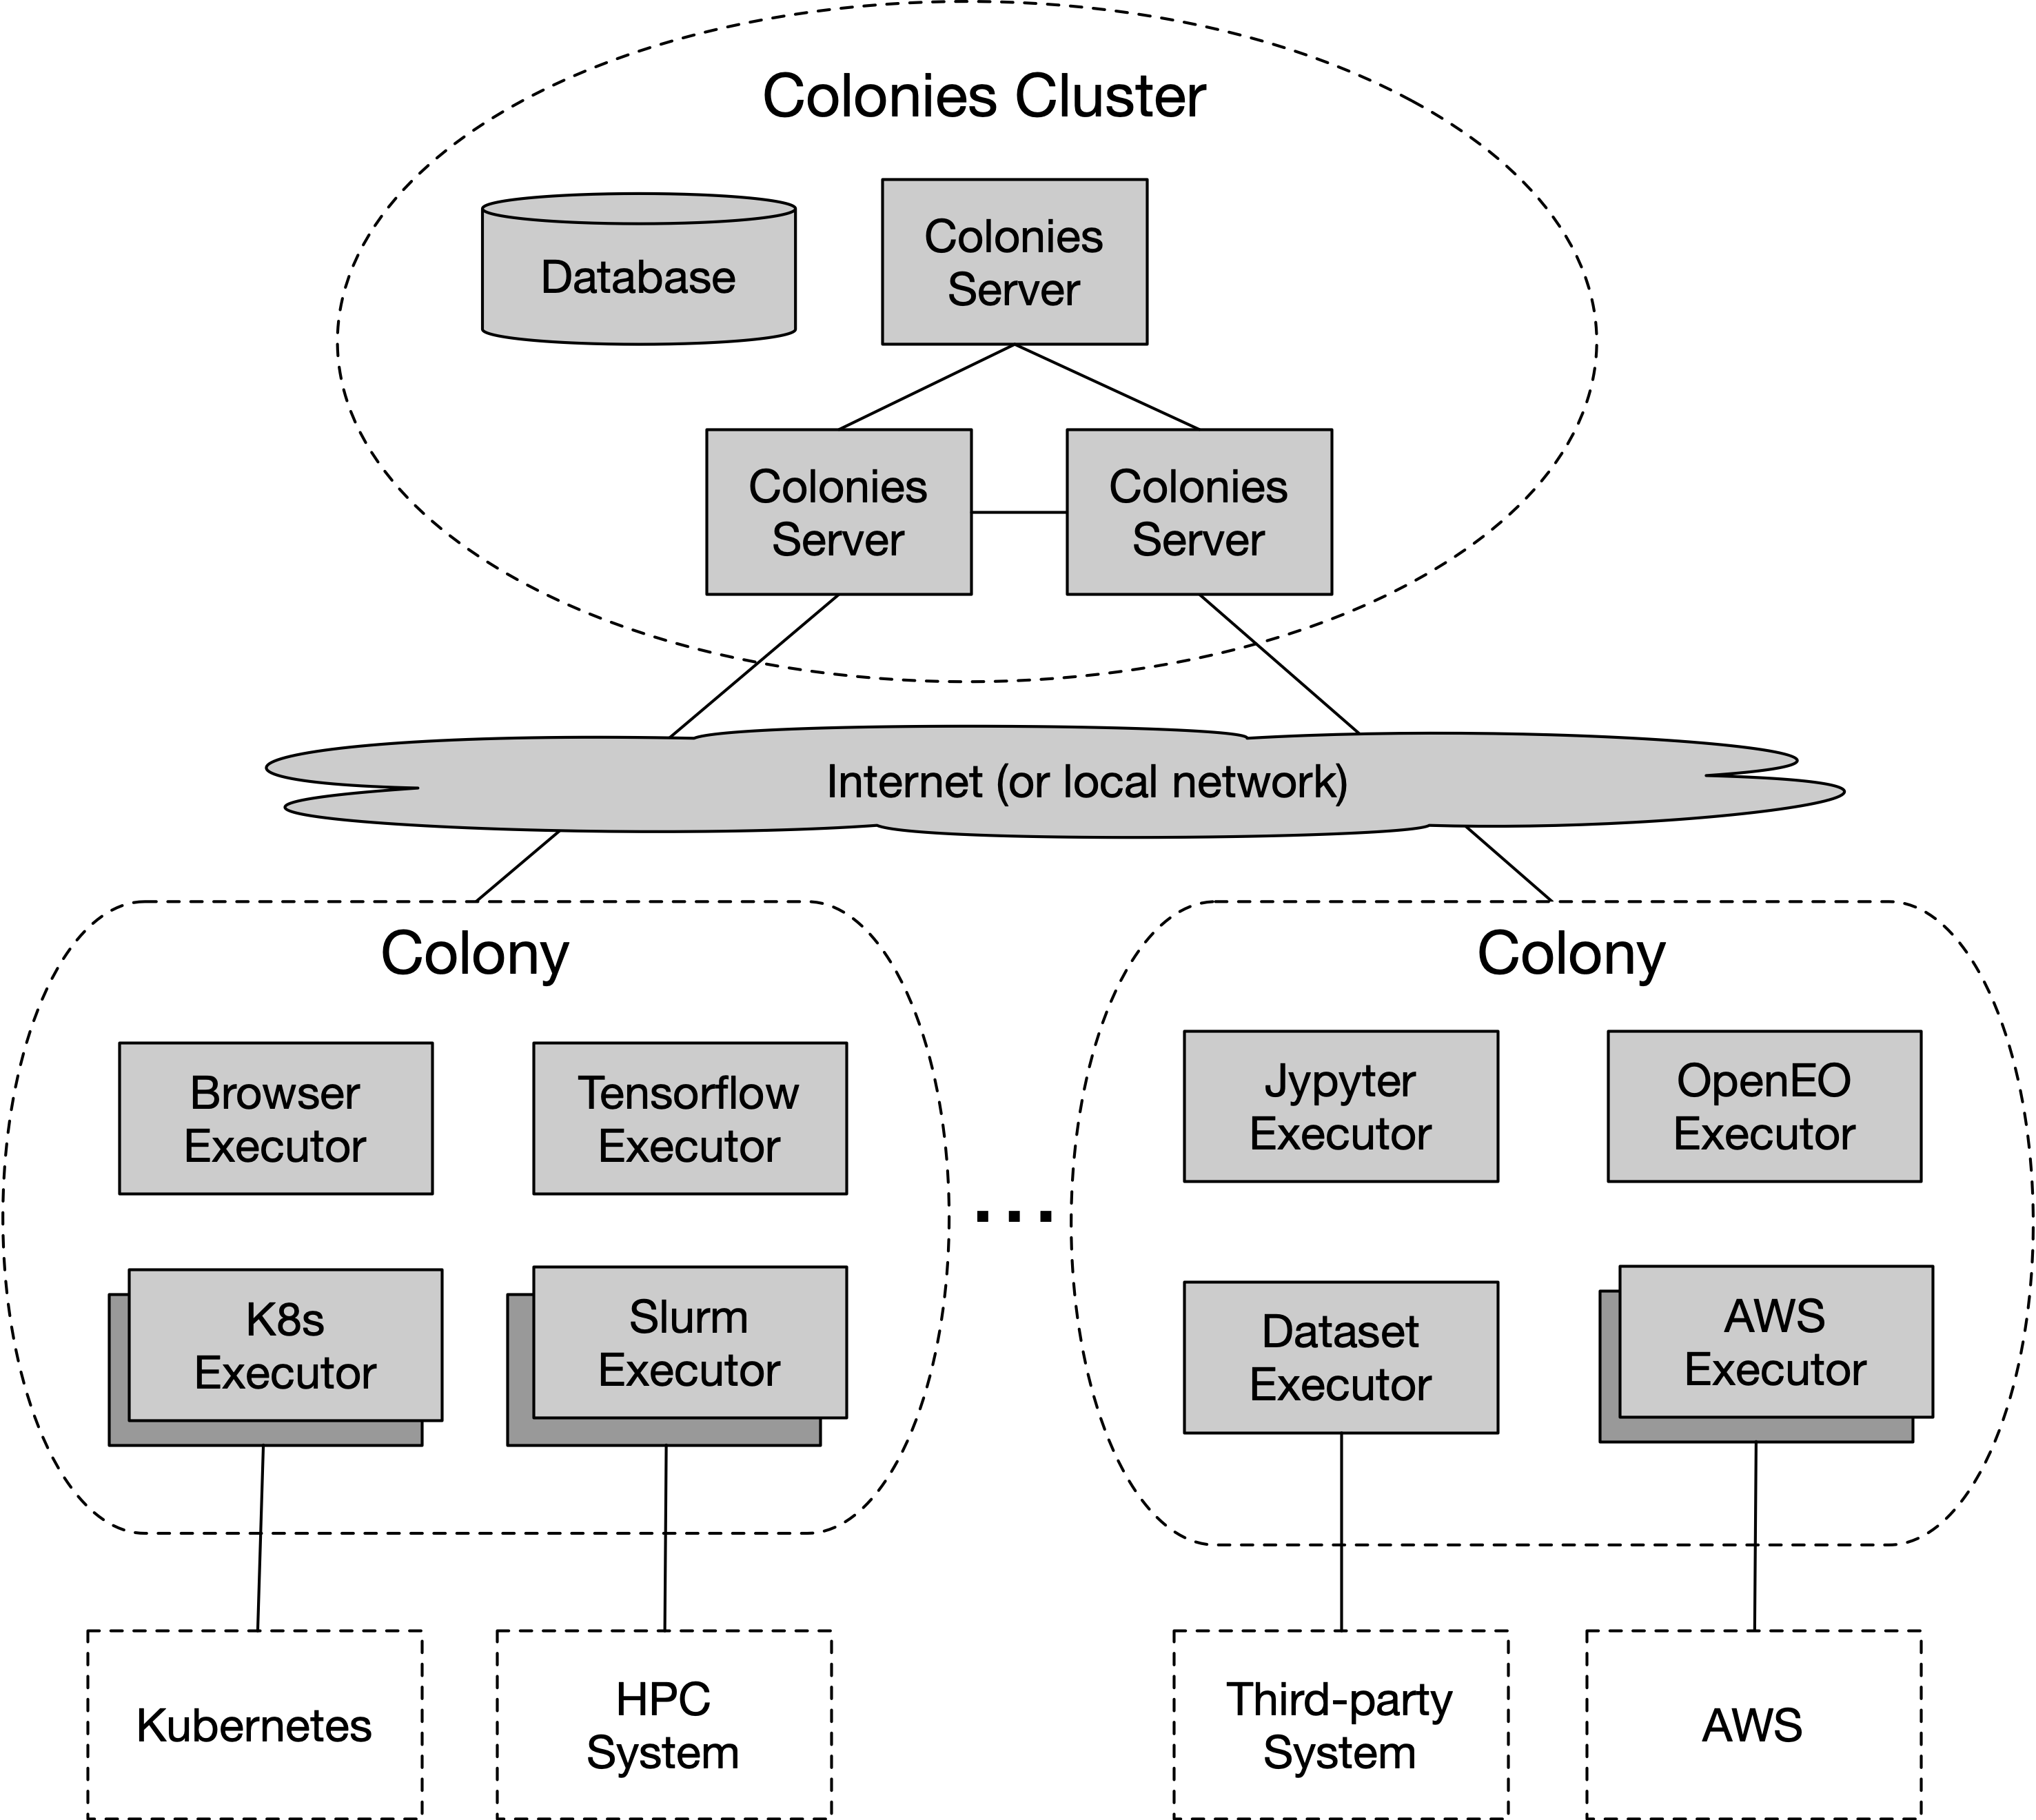
\includegraphics[scale=0.45]{overview.png}
	\caption{Overview of the Colonies framework. Executors may be deployed anywhere on the Internet.}
	\label{fig:overview}
\end{figure}

\section{The Colonies framework}
\label{sec:headings}
A core concept of the Colonies framework is the notion of \emph{processes}. A process contains meta-information about computations executed by remote computer programs, referred to as \emph{distributed executors}. Specifically, a process contains a definition of a function to be executed as well as contextual information such as execution status, including the result of the computation. One can think of a process as a digital twin of a real computing process. It is essential to note that a process does not necessarily have to be an operating system process, but can represent any type of computation, e.g. a remote procedure call executed by any kind of software. 

Figure 1 depicts an overview of the components part of the Colonies framework. The \emph{Colonies servers} form the backbone of the framework, functioning as a centralized control system for task submission and assignment. The Colonies server serves as a job broker for executors, almost like an employment agency for people. All execution information and history are stored in a database maintained by the Colonies servers. Upon submission, a process is stored in the database, serving as a queueing system. When a process is assigned to an executor its execution status is changed from \emph{waiting} to \emph{running}. Consequently, it is possible to submit a process that should run in the future even if no executors can run the process at the moment. In this way, Colonies supports both batch and real-time processing. 

\emph{Distributed executors} are responsible for executing processes assigned by the Colonies Servers. Several distributed executors form a \emph{Colony}, which is a collection of executors operating as a cohesive unit where each executor is responsible for executing specific types of processes. One could view a Colony as an organization or a society of distributed computer softwares acting as a single virtual computer system. To interact with other executors, executors must prove their Colony membership using a cryptographic protocol that follows the zero-trust security principle: \emph{never trust, always verify}. This security protocol ensures that users can keep control even when executors are distributed across platforms. Zero-trust security is fundamental to the Colonies framework and will be further discussed in Section \ref{zerotrustsecurity}. The following section outlines the underlying design principles and describe the Colonies framework in more detail. 

\subsection{Microservices}
Microservices \cite{microservices} is an architectural design pattern in which an application is structured as a collection of small, independently deployable, and loosely coupled services that communicate with other microservices through a well-defined API. By dividing the application into smaller, focused microservices, applications become easier to understand, maintain, and develop. In the Colonies framework, executors are microservices having the following characteristics:

\begin{itemize}
\item \textbf{Single responsibility:} Each executor is only accountable for executing specific functions. This makes the system easier to understand, develop, test and maintain.  
\item \textbf{Loosely coupled:} Executors are designed with minimal dependencies on other executors, enabling various software development teams to work independently. For instance, a data engineering team may handle the implementation of pre-processing functions, while a data science team oversees machine learning functions, and another team manages visualization or customer integration etc.

\item \textbf{Scalability:} Executors can be deployed independently, which enables horizontal scaling. This allows for better resource utilization, parallelism, and improved performance. 

\item \textbf{Resilience:} The failure of a single executor does not compromise the entire application or workflow. Executors' isolation from one another contributes to a more resilient and fault-tolerant system. If an executor crashes during execution, the process is automatically reassigned to another executor.

\item \textbf{DevOps and Continuous Integration:} Executors' inherent fault-tolerant design permits changes to individual executors without impacting the entire system. This makes it possible to seamlessly update the system. 

\item \textbf{Technology agnostic:} Executors can be implemented in any programming language, facilitating seamless integration with other applications and systems.

\item \textbf{Decentralized governance:} As the Colonies framework is technology-agnostic, different software development teams can make independent technology and design decisions when developing executors, promoting greater flexibility and adaptability. For example, some executors may be implemented in Rust, while others may use Python to leverage state-of-the-art machine learning frameworks.
\end{itemize}

Although microservices have attractive properties and can simplify both development and deployment of executors, they also introduce additional complexity that must be managed by the Colonies framework. To implement a workflow management framework supporting distributed microservices, the following challenges must be addressed:

\begin{itemize}
\item \textbf{Process management:} Colonies must be able to distribute processes among available executors based on their capabilities and current workload. This involves assigning processes to the most appropriate executor and then monitoring execution progress.

\item \textbf{Fault tolerance and recovery:} In the event of executor failures, the Colonies framework must be able to re-assign processes to other executors, manage executor restarts, or trigger recovery mechanisms to maintain system reliability and resilience. In addition, the Colonies framework must be able to handle restarts or crashes of Colonies servers, thereby preventing any internal states in Colonies from becoming corrupted. 

\item \textbf{Load balancing:} The Colonies framework must manage load balancing among executors to optimize performance and avoid overloading any single executor.

\item \textbf{Service discovery:} The Colonies framework must enable executors to dynamically register and deregister from Colonies servers. It must be possible to deploy executors anywhere on the Internet, even behind firewalls.

\item \textbf{Workflow orchestration:} The Colonies framework must coordinate and orchestrate complex multi-step workflows executed by several executors, sometimes in parallel where executors run on different platforms. Colonies must define the sequence in which processes should be executed, manage dependencies among processes, and ensure that workflows execute successfully to completion.

\item \textbf{Monitoring and debugging:} The Colonies framework must monitor the overall system, allowing administrators to track the health, performance, and resource utilization of the executors and the system as a whole.
\end{itemize}

The Colonies framework uses a combination of technologies to address the aforementioned challenges. A fundamental design principle is statelessness, which makes Colonies simpler, more reliable and scalable, and easier to implement. To ensure reliability and data consistency, a distributed consensus algorithm is needed to handle high-availability and server crashes. The remainder of this section describes how the Colonies framework is implemented. The next discusses the role of queues to support batch jobs and realtime processing, but also queues roles in implementing loosely coupled systems.

\begin{figure}
     \centering
     \begin{subfigure}[b]{0.4\textwidth}
         \centering
         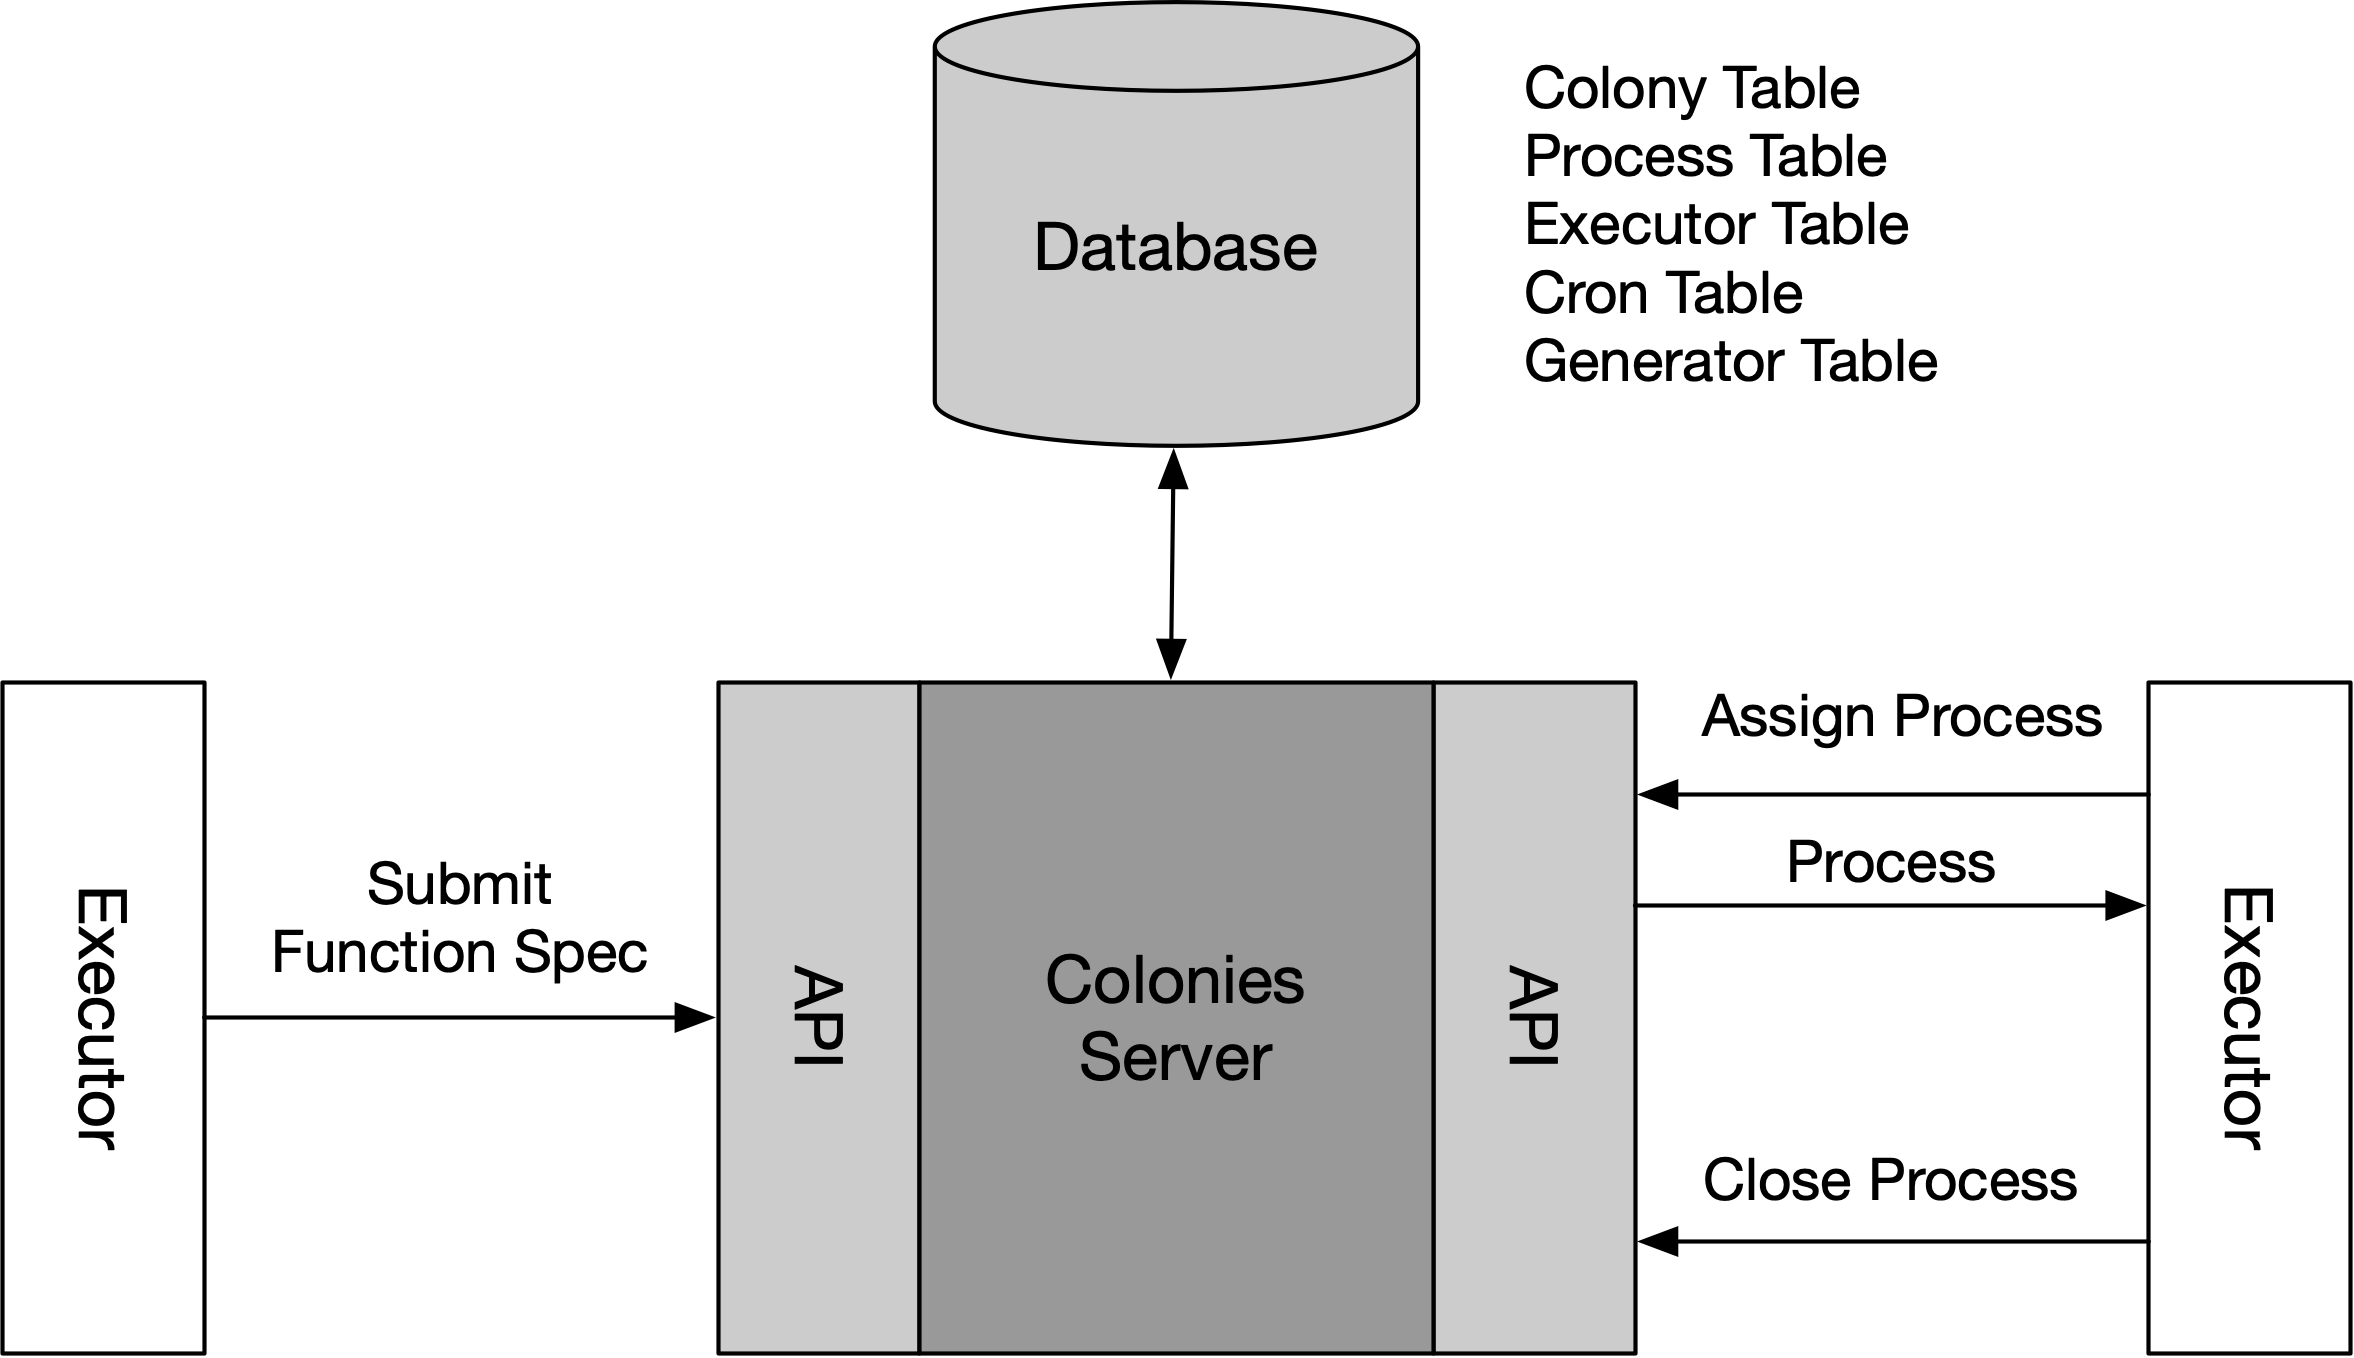
\includegraphics[scale=0.45]{arch.png}
         \caption{Process assignment steps.}
     \end{subfigure}
     \hfill
     \begin{subfigure}[b]{0.4\textwidth}
         \centering
         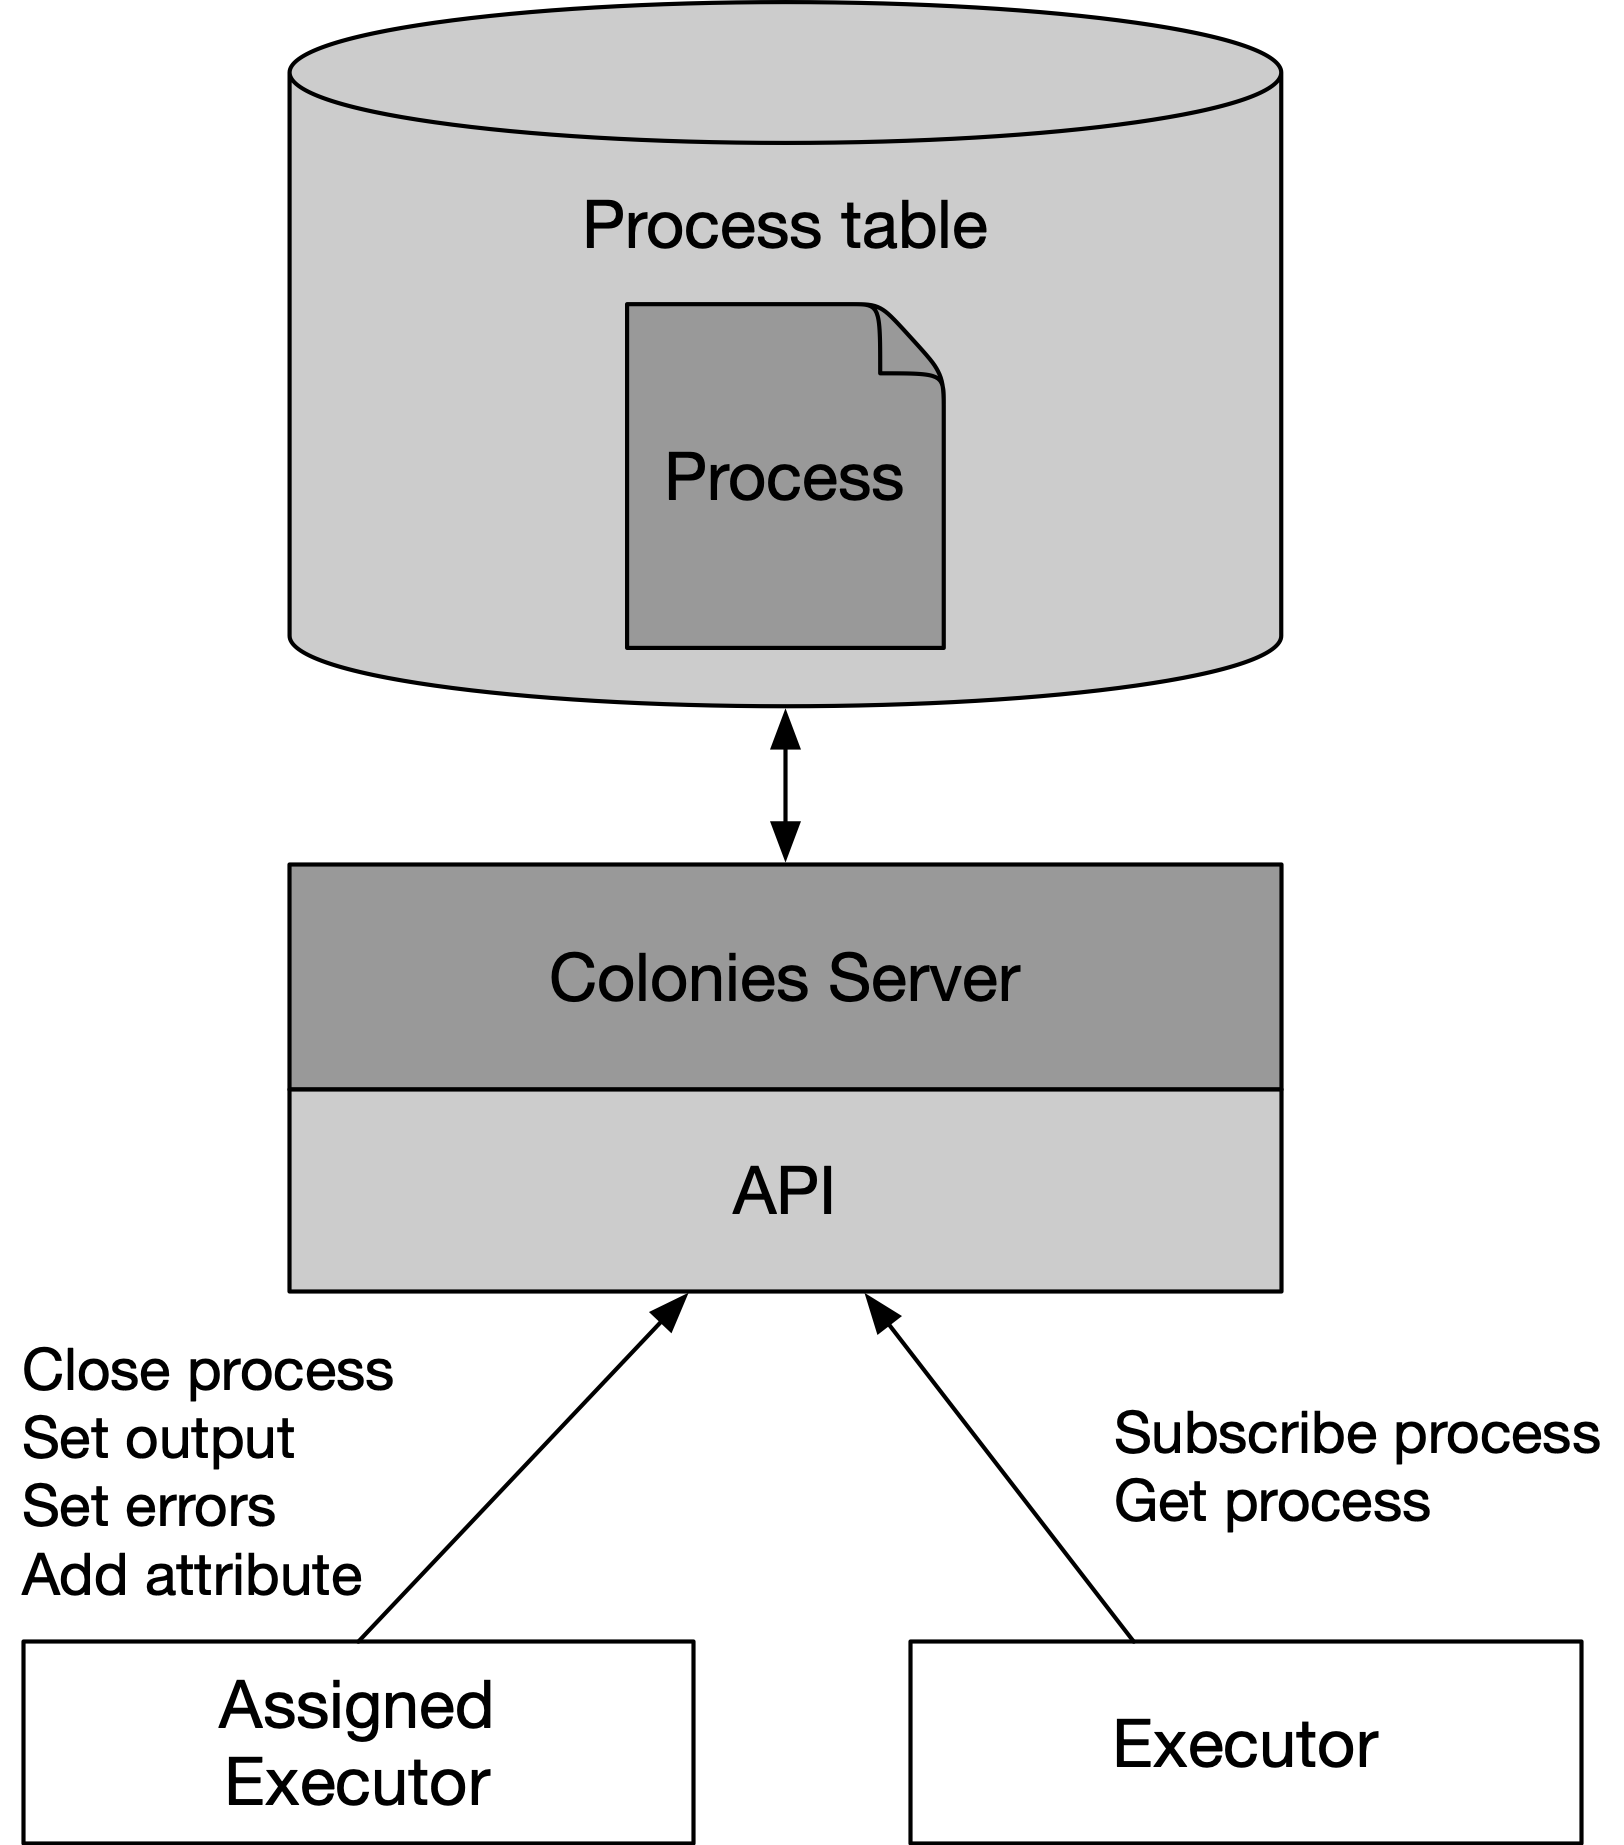
\includegraphics[scale=0.45]{process.png}
         \caption{Manipulation of a process.}
     \end{subfigure}
     \caption{Process management via Colonies HTTP API. Note that only the assigned executor has write access to the process database entry.}
     \label{fig:process_assignment}
\end{figure}

\subsection{The role of queues as seperation of concerns}
Separation of concerns (SoC) is a design principle to break down a complex software system into smaller, more manageable parts. For example, HTTP APIs can be used to abstract away implementation detail and provide a clear and simple interface for interacting with a particular service. However, HTTP APIs alone are insufficient for handling dynamic environments where components frequently fail or the underlying infrastructure is constantly changing. To address such environments, an alternative mechanism is needed. 

Queues enable software services to communicate indirectly by acting as a buffer between them. Queues make it possible to decouple executor and make them operate independently, for example an executor can be updated or replaced without affecting other executors. Queues also enable asynchronous communication between executors, enabling them to process tasks at their own pace. This ensures that slower executors do not bottleneck faster ones, leading to a more efficient and scalable system. Most importantly, queues enable load balancing by distributing tasks among executors, thus making it possible to parallelize workflow execution. 

Queues can be implemented in different ways. While message brokers are a common solution, Colonies adopt an alternative strategy and leverage a standard database and query it for processes to assign to different executors. One key advantage of this approach is that it enables fine-grained process assignments, making it possible to assign specific processes to particular executors. For instance, an executor of the browser type can be limited to only executing processes capable of running in web browsers. This level of granularity cannot easily be implemented using message brokers which generally do not offer introspection of queues, or provide the ability to pull specific messages out of the queue. Generally, the only way to retrieve a specific message is to pull all messages from the queue, obtain the message, and then place all remaining messages back into the queue in the same order. In contrast, a database can function as a queue and a query can match any columns making it possible to assign specific executors to specific processes.

\subsection{Process tables}
Colonies enables executors to interact with each other by submitting function specifications to the Colonies servers. Once submitted, other executors can connect to the servers to receive process execution assignments. A new process entry is automatically added to the process table database when a function specification is submitted to the Colonies server.

\begin{table}[t]
	\caption{Process Table}
	\centering
	\begin{tabular}{llllll}
		\toprule
		\cmidrule(r){1-2}
        Process Id & Function Spec & Wait for Parents & Executor  & State      & Priority Time \\
		\midrule
        $P_{1}$    & $F_{1}$       & $False$          & $E_{1}$   & Successful & 1679906715352024000 \\
        $P_{2}$    & $F_{2}$       & $False$          & $E_{1}$   & Running    & 1679906715353453000 \\
        $P_{3}$    & $F_{3}$       & $False$          & $E_{2}$   & Running    & 1679906715354286000 \\
        $P_{4}$    & $F_{4}$       & $True$           & -         & Waiting    & 1679906715355188000 \\
		\bottomrule
	\end{tabular}
	\label{proctable}
\end{table}

\begin{table}[t]
	\caption{Function Specifications}
	\centering
	\begin{tabular}{llllll}
		\toprule
		\cmidrule(r){1-2}
        Function Spec & Function        & Executor Type & Priority & Max Exec Time & Max Retries \\
		\midrule
        $F_{1}$       & gen\_nums()     & Edge          & 1        & 200 s         & 5 \\
        $F_{2}$       & square()        & Cloud         & 1        & 200 s         & 5 \\
        $F_{3}$       & square()        & Cloud         & 1        & 200 s         & 5 \\
        $F_{4}$       & sum()           & Browser       & 1        & 200 s         & 5 \\
		\bottomrule
	\end{tabular}
	\label{functable}
\end{table}

When an executor connects to the Colonies server, the server hangs the incoming HTTP connection\footnote{An alternative protocol is to use WebSockets or gPRC to communicate with the Colonies server.} until the executor is assigned a process, or until a connection timer expires. The Colonies server never connects to the executors. Rather, it is the responsibility of the executors to connect to the Colonies server. This enables executors to be deployed anywhere on the Internet, behind firewalls, commercial telco networks, or even in web browser-based applications.

\begin{lstlisting}[basicstyle=\small, label=fig:function_spec, language=json, basicstyle=\small, caption=Example of a function specification.]
{
   "conditions": {
       "colonyid": "0c1168fe986ffe39fad14f17e0bd9e5896f6d968405ac0fb3380154109ee4022",
       "executortype": "helloworld_executor"
   },
   "funcname": "helloworld",
   "args": ["hello world"],
   "maxwaittime": 10,
   "maxexectime": 100,
   "maxretries": 3,
   "priority": 1
}
\end{lstlisting}

Figure \ref{fig:process_assignment} depicts an executor submitting a function specification that is later assigned to another executor. When registering, executors have to specify to the Colonies server which functions they are capable of executing. The Colonies server then makes sure that the conditions part of the function specification matches the capability of an executor. 

\begin{equation}
    \label{eq:pt}
    priority_{time}=submission_{time} - priority \cdot 10^9 \cdot 60 \cdot 60 \cdot 24
\end{equation}

Table \ref{proctable} shows an example of a process table. The process table also contains a reference to a function specification depicted in Table \ref{functable}. To assign a process to an executor, the Colonies server searches in the process table to find a process matching a waiting executor. By using the \emph{priority time} column to sort the processes, the process table can function as a queue. This can be done in SQL by utilizing the \emph{order by} clause to sort processes according to their submission time. 

To make it possible to handle priorities, the submission time is adjusted so that higher priority processes are processed before lower priority processes. When a process is submitted, a \emph{priority time} value is calculated and stored in the process table. Equation \ref{eq:pt} shows how the priority time is calculated for a nanosecond timestamp. 

\begin{figure}[h]
	\centering
    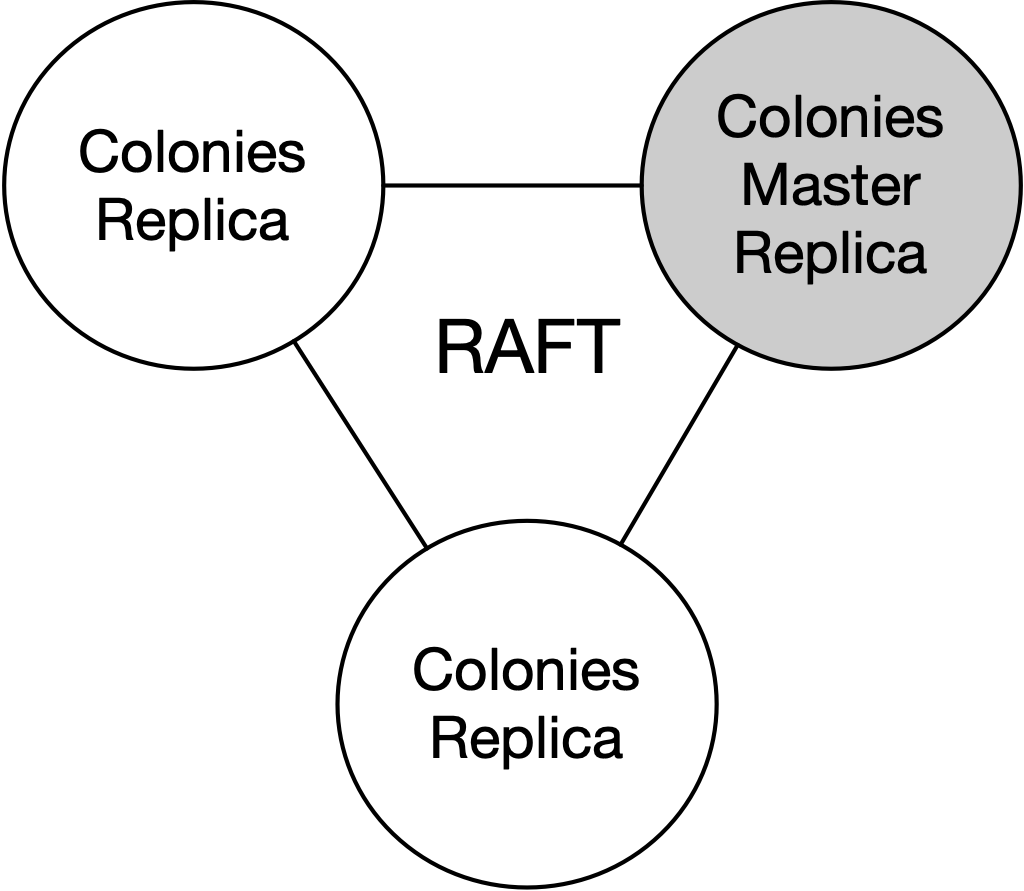
\includegraphics[scale=0.5]{raft.png}
	\caption{High-availability deployment of Colonies.}
	\label{fig:ha_deployment}
\end{figure}

\subsection{A stateless failsafe mechanism}
\label{stateless_error_management}
The primary objective of all Colonies API requests is to alter some state stored in the database or retrieve information from the database. The Colonies framework is designed to be stateless, meaning that Colonies servers do not keep any information in memory between requests. Each request is handled independently without relying on information from previous requests. 

Figure \ref{fig:function_spec} shows an example of a function specification. The \emph{maxexectime} attribute specifies the maximum time an executor may run a process (in this case, 100 seconds). Before a process is assigned to an executor, the Colonies server updates the process entry in the process table database and calculates a deadline when the process must be finished. The server then regularly checks for any running processes that have exceeded their deadlines. If such a process is detected, it is reset, allowing it to be re-assigned to other executors. 

Making it possible to specify maximum execution time is a simple but powerful mechanism. To scale up a system, more executors can simply be deployed. Scaling down, however, can be more challenging. One solution is to select a set of executors to be removed and then starve them out by denying them new process assignments. Another, simpler solution, is to immediately destroy the executors and use the \emph{maxexectime} failsafe mechanism to move back processes from defunct executors to the queue. The \emph{maxexectime} failsafe mechanism ensures that processes will eventually be executed even in the case of failures. This mechanism also relieves the burden of the user to check if a process has been executed or not, as they can simply look up the process in the database to get its current status. 

Utilizing the \emph{maxexectime} failsafe mechanism not only enhances system reliability, but also provides an opportunity to apply Chaos engineering \cite{chaos_engineering}. For example, a Chaos monkey can be used to deliberately terminate executors. If executors are deployed on Kubernetes, Kubernetes will then automatically redeploy terminated executors. The constant flux of executor replacements ensures that the system is capable of gracefully tolerating failures.

\subsubsection{Data consistency and distributed consensus}
Synchronization is essential to prevent data inconsistency and race conditions when accessing shared resources concurrently with multiple threads. However, synchronization can also slow down execution as only one thread can access critical sections at a time. By carefully designing multithreaded applications and using right synchronization techniques, it is possible to minimize the performance impact while still ensuring data consistency and correctness.  

The \emph{assign} API request binds a process from the database to an executor. Given the multi-threaded nature of the Colonies server, it is essential that the \emph{assign} request is synchronized to ensure that only one thread at a time can modify the database and update the process table, thus preventing multiple executors from being assigned to the same process. To ensure that only one executor can be assigned to a process, the \emph{assign} request must be synchronized. It is worth noting that synchronization is not necessary for other requests. For example, as the \emph{submit} request only adds new entries to the process table, there are no race conditions. The \emph{close} request sets the output of the function innovation and updates the process state to either successful or failed in the process table. Since there can only be one executor assigned to a process there are no race conditions and consequently no need for synchronization.

To minimize downtime, Colonies supports high-availability deployments. If one Colonies server crashes, an executor simply need to resend the failed request, which will then be served by another Colonies server replica. However, by introducing multiple Colonies servers, there is again a risk of race conditions when assigning processes to executors. This means that the Colonies must coordinate which replica server should serve incoming assign requests so that precisely one executor is assigned to a particular process.

Raft \cite{raft} is a consensus algorithm specifically designed to manage a replicated log within a distributed system. Raft makes it possible to implement distributed leader elections where a single server takes on the role of leader while the remaining servers act as followers. The leader is responsible for managing the replicated log, processing client requests, and replicating entries to the followers. Followers passively replicate the leader's log and participate in leader elections. 

By using the Raft protocol, Colonies can redirect incoming \emph{assign} requests to the leading Colonies server, thereby ensuring that only one Colonies server replica handles assign requests. A new leader is automatically elected in the event that a Colonies server replica fails. Figure \ref{fig:ha_deployment} shows an overview of a high-availability Colonies deployment. In addition, the Raft protocol makes it possible to seamlessly update Colonies software by making it possible to upgrade each Colonies server replica individually. Consequently, making Colonies servers well-suited for Kubernetes deployments.

\begin{table}[h]
	\caption{Dependency Table}
	\centering
	\begin{tabular}{lll}
		\toprule
		\cmidrule(r){1-2}
        Process Id & Name       & Dependencies           \\
		\midrule
        $P_{1}$    & $Task_{1}$ & -                      \\
        $P_{2}$    & $Task_{2}$ & $Task_{1}$             \\
        $P_{3}$    & $Task_{3}$ & $Task_{1}$             \\
        $P_{4}$    & $Task_{4}$ & $Task_{2}$, $Task_{3}$ \\
		\bottomrule
	\end{tabular}
	\label{deptable}
\end{table}

\subsubsection{Workflows}
A workflow is a series of processes that need to be completed in a specific order. In Colonies, workflows are represented as directed acyclic graphs (DAGs) where nodes represent processes and edges represent dependencies and data flow between processes. Similar to processes, workflows are managed completely stateless. When a workflow is submitted, all processes part of the workflow are submitted and added to the process table similar to how ordinary processes are handled. To control the order processes can be assigned, Colonies sets a flag, \emph{wait for parents} to prevent processes to be assigned to an executor before their dependencies have been satisfied. Note that processes may run in parallel if a sufficient number of executors are available, assuming their parent processes have finished.


\begin{figure}[h]
	\centering
    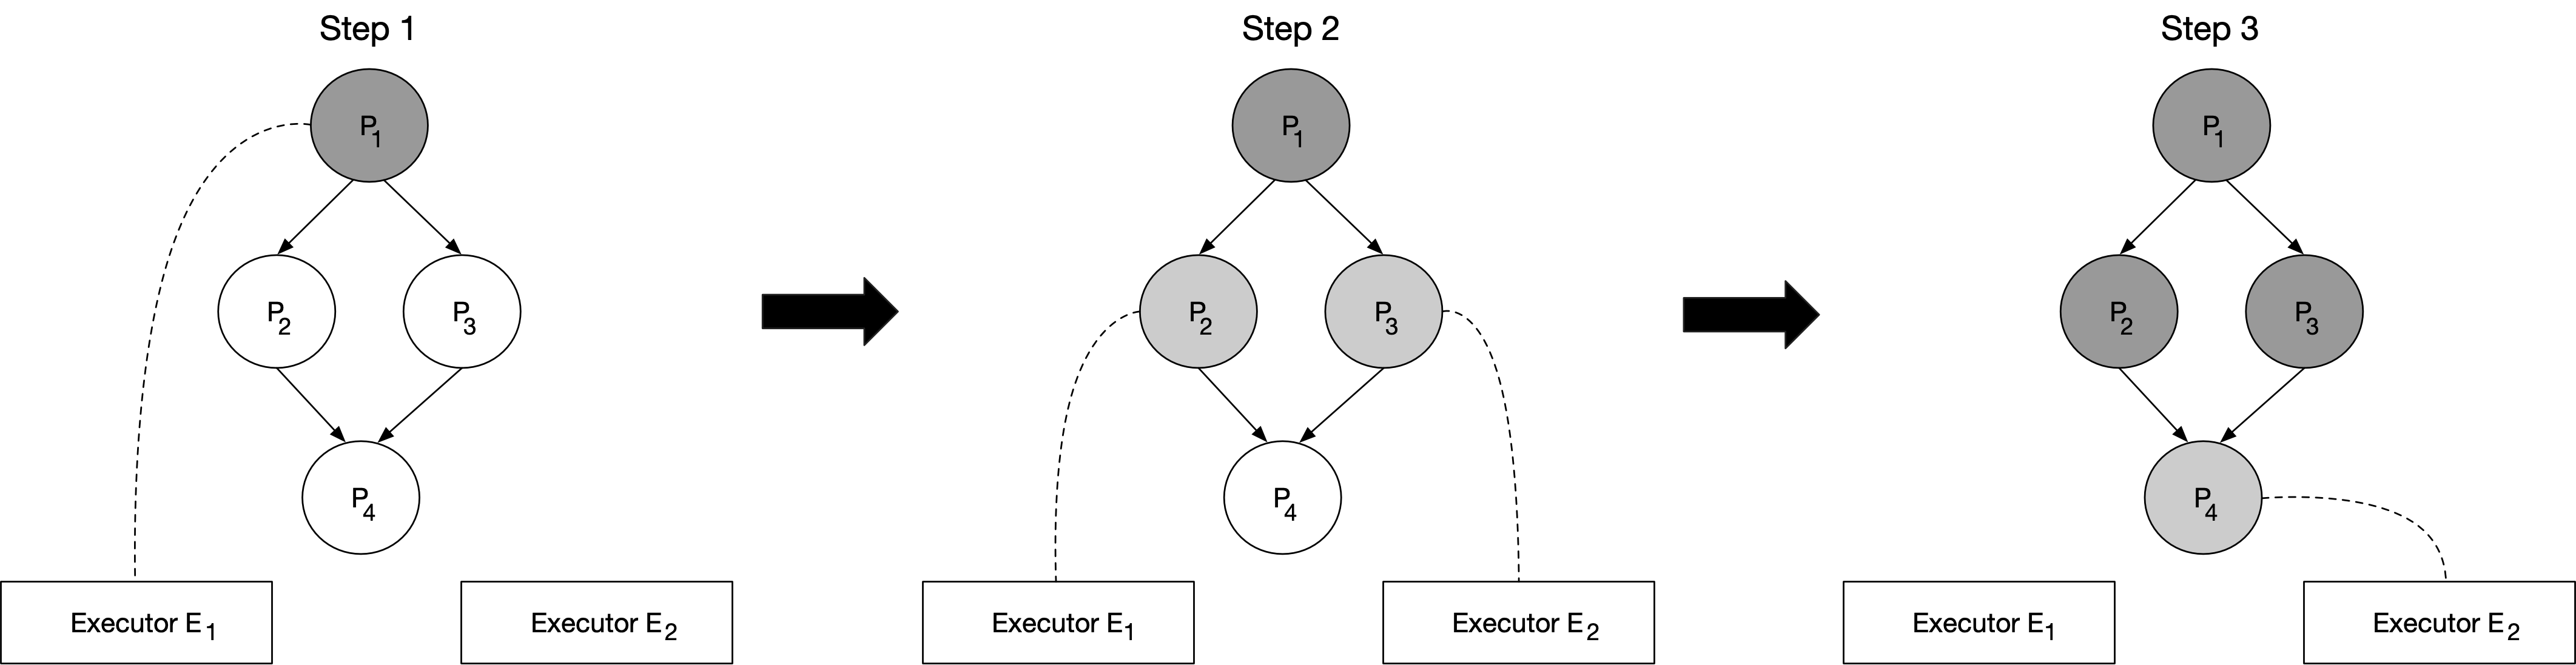
\includegraphics[scale=0.30]{workflow.png}
	\caption{Workflow execution timeline.}
	\label{fig:workflowexec}
\end{figure}

When a process is closed, the Colonies server checks its child processes to see if all their parent processes have also completed. If all parents of a child process have finished, the server updates the process table in the database by setting the flag \emph{wait for parents} to \emph{false}, which allows child processes to be assigned to executors. This operation is also done statelessly when processing the \emph{close} request. 

Figure \ref{fig:workflowexec} shows an execution timeline for a workflow. Upon submission, process \(P_{1}\) is assigned to Executor \(E_{1}\). After being closed, processes \(P_{2}\) and \(P_{3}\) are simultaneously assigned to \(E_{1}\) and \(E_{2}\), allowing for concurrent execution. Lastly, process \(P_{4}\) is assigned to \(E_{2}\).  

To be able to generate a DAG, an additional database table is required. Table \ref{deptable} shows an example of a dependency table storing relationships between processes. The table is updated when a workflow is submitted to a Colonies server. As mentioned before, when an executor is assigned a process, it obtains exclusive rights to that process within the process table. This exclusivity also means that it is possible for an exector to dynamically add new children processes to the workflow DAG on the fly. As a result, it becomes possible to implement MapReduce \cite{mapreduce} data processing patterns similar to Hadoop \cite{hadoop}.  

\begin{table}[h]
	\caption{Input/Output}
	\centering
	\begin{tabular}{lll}
		\toprule
		\cmidrule(r){1-2}
        Process Id & Input & Output \\
		\midrule
        $P_{1}$    & & [2,3] \\
        $P_{2}$    & 2 & 4 \\
        $P_{3}$    & 3 & 9 \\
        $P_{4}$    & [4,9] & 13 \\
		\bottomrule
	\end{tabular}
	\label{inouttable}
\end{table}

To manage data flow between processes that are part of a workflow, it is necessary to store the input and output values resulting from function invocations in a database. An example of such a database is presented in Table \ref{inouttable}. An executor can subsequently query the output from a parent process and use that as arguments while invoking a function.

\subsubsection{Cron}
The Colonies framework is based on a stateless architecture where each request is treated as an independent transaction which is processed without any information from prior requests. Since there is no session data stored in memory, Colonies can easily switch between servers without disruptions or data losses. In a stateful architecture on the other hand, the server must maintain a record of connected clients' state and session data in memory, which can result in complications if a server fails or crashes. 

Cron is a time-based job scheduler designed to trigger workflows at predefined intervals. It can for example be used to automate tasks such as routinely fetching data from external systems. To make Colonies robust and easy to implement, it is essential that Cron workflows also are managed stateless. This can be achieved by introducing an additional database table to store information about Cron workflow, and let the elected Colonies server leader assume the responsibility of managing Cron workflows through a two-step process. 

Firstly, the leading Colonies server calculates a future deadline, indicating when a specific Cron workflow is scheduled to be executed. The leader server then conducts periodic scans of the Cron table. When the current time surpasses the calculated deadline for a particular workflow, a new workflow is automatically submitted. Note that this protocol is completely stateless as no session information is stored in memory between cron scans. In the event that the leader Colonies server experiences a crash, a new leader is selected and assumes the responsibility of managing Cron workflows according to the two-step protocol.

\subsubsection{Generators}
Another feature of the Colonies framework are so-called generators. Generators are workflow templates that are automatically triggered when specific conditions are met. Generators can be used to accumulate input data into bulks to improve performance or parallelism. For example, an external service downloads satellite images and can use a generator to automatically triggered a workflow when 10 images are collected. This is achieved by sending a special \emph{pack} request containing input data to a Colonies server, targeting a certain generator. 

Generators facilities integration with third-party systems as it allows for stateless implementation where interactions with Colonies can be done in a fire-and-forget style. Colonies guarantees that all pack requests submitted to a generator are processed correctly, even if a Colonies server is restarted or fails. Without this robustness guarantee, third-party integration software would have to use an alternative method such as a message broker or a database to enqueue input data and periodically empty the queues to generate workflows themselves. This adds complexity to the integration process and may require additional infrastructure components. Generators are a powerful feature of the Colonies framework that can help simplify integration and implement robust data processing pipelines.

Generators can be implemented using a similar method to how Cron workflows are implemented. The elected leader Colonies server takes on the responsibility for scanning a special generator table to decide if a workflow should be triggered. This approach ensures that there is a single point of control for generating workflows and prevents generation of duplicate workflows. If the leader server crashes, a new leader Colonies server is automatically elected, which takes over the responsibility for triggering generators. This ensures that the generation of workflows is not impacted by server failures, and the system can continue to operate smoothly even in case of failures. It can be worth pointing out that since the \emph{pack} request only adds information to the generator table and does not manipulate any states, it can be processed by any Colonies server without synchronization precautious. This means that any Colonies server in the cluster can handle incoming \emph{pack} requests, which increases the scalability and fault-tolerance of the system as a whole.

\subsubsection{Zero-trust security}
\label{zerotrustsecurity}
As executors may be deployed across multiple platforms, there is a need for a unified security model that can be applied on top of any platform. Zero-trust security \cite{zerotrust} is a security model that assumes that any device or user is a potential threat, even if they are located within a secure network perimeter. Therefore, zero-trust security requires that every interaction between clients and servers is verified and authenticated before being processed, making it ideal for heterogeneous platform deployments. However, there must be a way to verify the identities of the clients to determine whether they should be granted access.

As previously stated, a colony is a collection of distributed executors. Executors part of the same colony trust each other and can thus submit function specifications and get process execution assignments. To implement such a scheme, the Colonies server must be able to verify the identity of the executors and then check their colony membership. This can be accomplished in various ways. One solution is to use public key encryption and assign each executor a pair of keys - a public key and a private key. The public key is openly available and uploaded to the Colonies server, whereas the private key is kept secret and is only used by the executor to sign API request messages. The Colony server can then verify the signature of incoming request messages and use the public keys to determine whether an executor is a member of a certain colony.

ECDSA (Elliptic Curve Digital Signature Algorithm) \cite{ecdsa} is a digital public key encryption signature algorithm. It is widely used in blockchains such as Bitcoin and Ethereum to verify transactions. One of the advantages of ECDSA is its ability to recover public keys from received messages and signatures without explicitly transmitting the public keys. This is particularly useful as the identity of an executor can be calculated simply as the SHA-3 hash of the recovered signature, saving space and eliminating the need for storing public keys. 

In Colonies, there exist three distinct roles, each with its own set of responsibilities and authority levels. The Colonies server owner holds the highest level of authority and has permission to add new colonies to the Colonies server. The colony owner is responsible for the management of a given colony and has permission to register or unregister executors within that colony. Executors, on the other hand, have the lowest level of authority and are only authorized to manage processes within their appointed colony. This functionality can be implemented by introducing a new table to the Colonies database, the colony table.

\begin{table}[h]
    \caption{Colony Id: \(4787a5071856a4acf702b2ffcea422e3237a679c681314113d86139461290cf4\)}
	\centering
	\begin{tabular}{ll}
		\toprule
		\cmidrule(r){1-2}
        Executor Id & Executor Name \\
		\midrule
        \(8a491bcac0be623a54411dd0934fdcdc9c844de5700527a7dbc9da08a6a8310d\) & $E_{1}$ \\
        \(6a65f40343999415f47e739f09b625ab437b069b5f591f9844c234533f505bee\) & $E_{2}$ \\
        \(41e4c1b10f92a53b7a5a86620ed366635901a1a96c48312a0ef566a13217fe03\) & $E_{3}$ \\
		\bottomrule
	\end{tabular}
	\label{coltable}
\end{table}

Table \ref{coltable} shows an example of a colony table consisting of three executors. In this case, to register a new executor, the SHA-3 hash of the recovered signature needs to match the identity \(4787a5071856a4acf702b2ffcea422e3237a679c681314113d86139461290cf4\) stored in the colony table. This operation can only be performed by the colony owner possessing the corresponding private key. Similarly, when an executor connects to the Colonies server to either submit a function specification or get a process assignment, it needs to sign the API message with its private key. The Colonies server will then recover the identity of the executor and look up the colony table to check if the executor is a rightful colony member. See Appendix A for additional details on how the various roles apply to different Colonies operations.

An advantage of using a stateless architecture for workflow management as proposed in the paper is the ability to monitor executor performance to detect any unusual or suspicious behaviors. Because the execution history is recorded in a database, it is possible to track the activity of individual executors and identify any unusual patterns. For example, if an executor suddenly starts to consume a lot of resources, it could indicate a performance issue or it could be a sign of malicious activity, such as a denial-of-service attack. Automatic monitoring can for example be implemented using anomaly detection algorithms and machine learning to grade the performance of each executor. Administrators can then be automatically notified if the grade of an executor exceeds a certain threshold, enabling them to take appropriate actions.

\section{Implementation}
Colonies is implemented in Golang and is publicly available on GitHub\footnote{https://github.com/colonyos/colonies} under the MIT license. It consists of a statically compiled binary that offers a CLI tool for deploying Colonies servers or managing the system. Furthermore, there are several software development kits (SDKs) available for various programming languages, including Golang\footnote{https://github.com/colonyos/colonies/tree/main/pkg/client}, Rust\footnote{https://github.com/colonyos/rust}, Julia\footnote{https://github.com/colonyos/Colonies.jl}, JavaScript\footnote{https://github.com/colonyos/colonies.js}, Python\footnote{https://github.com/colonyos/pycolonies}, and Haskell\footnote{https://github.com/colonyos/haskell}. As an introduction to Colonies, the following section gives a brief overview how to use the Python SDK.

\subsection{Python SDK}
A Colonies application typically consists of a set executors written in different programming languages and deployed across multiple platforms. The executors are small microservices that interact with one another by submitting function specifications or workflows, which are then executed by other executors that are part of the same colony.

The first step in implementing an executor in Python is to create a private key and identity, followed by registering the executor with a colony. As mentioned before, executor can registration can only be carried out by the colony owner using the colony private key. Code in Listening \ref{code:regexecutor} illustrates how to register an executor, including registering functions a specific executor is capable of running. In the example, an executor of type \emph{helloworld\_executor} is registered to run a function named \emph{helloworld}.

\begin{lstlisting}[showstringspaces=false, frame=lines, numbers=left, numberstyle=\scriptsize, backgroundcolor=\color{background}, basicstyle=\small, label=code:regexecutor, language=Python, caption=Register an executor to a colony in Python.]
colonies = Colonies("localhost", 50080)

crypto = Crypto()
colonyid = "4787a5071856a4acf702b2ffcea422e3237a679c681314113d86139461290cf4"
colony_prvkey = "ba949fa134981372d6da62b6a56f336ab4d843b22c02a4257dcf7d0d73097514"
executor_prvkey = crypto.prvkey()
executorid = crypto.id(executor_prvkey)

executor = {
    "executorname": "helloworld_executor",
    "executorid": executorid,
    "colonyid": colonyid,
    "executortype": "helloworld _executor"
}

colonies.add_executor(executor, colony_prvkey)
colonies.approve_executor(executorid, colony_prvkey)

# register capability run the helloworld function
colonies.add_function(executorid, colonyid, "helloworld",  executor_prvkey)
\end{lstlisting}

After registration, the executor must connect to the Colonies server and request process assignments of the type \emph{helloworld\_executor}. Note that executor properties, such as the executor type, are not explicitly set in the \emph{assign} request, but rather derived implicitly by the Colonies server from the executor identity, which is derived from the signature generated by the executor's private key. This approach ensures that the executor can only be assigned processes that match its registered capabilities.

\begin{lstlisting}[showstringspaces=false, frame=lines, numbers=left, numberstyle=\scriptsize, backgroundcolor=\color{background}, basicstyle=\small, language=Python, label=code:assign, caption=Assigning and executing a process in Python.]
while True:
    process = colonies.assign(colonyid, 10, executor_prvkey)
    if process["spec"]["funcname"] == "helloworld":
       colonies.close(process["processid"], ["hello world"], executor_prvkey)
\end{lstlisting}

This \emph{assign} request is always initiated by the executor, allowing executors to be deployed behind firewalls. When receiving the request, the Colonies server hangs the request until a matching process is found or a timer expires. In the example in Listing \ref{code:assign}, the timer is set for 10 seconds, after which an exception is raised, and the executor must reconnect to the server.

When assigned to a process, the executor interprets the metadata stored in the process data structure, including the function name and arguments, and performs some kind of computation such as preprocessing data or training a neural network. Upon completion, the executor closes the process and sets the output. In the example, the output is set to the string \emph{helloworld}.

\begin{lstlisting}[showstringspaces=false, frame=lines, numbers=left, numberstyle=\scriptsize, backgroundcolor=\color{background}, basicstyle=\small, language=Python, label=code:submit, caption=Submitting a function specification.]
func_spec = create_func_spec(func="helloworld",
                             colonyid=colonyid,
                             executortype="helloworld_executor",
                             priority=0,
                             maxexectime=100,
                             maxretries=3)
process = colonies.submit(func_spec, executor_prvkey)
\end{lstlisting}

Listing \ref{code:submit} demonstrates how to submit a function specification using the Python SDK and call the \emph{helloworld} function. Note that the executor must complete the process within 100 seconds. The process is reassigned to another executor if the execution takes too long a time. The previous executor then receives an error when trying to send a \emph{close} request. As discussed in Section \ref{stateless_error_management}, establishing boundaries on computations is critical to achieving robustness and supporting infrastructural changes that may result from DevOps or IT operations.

\begin{figure}
     \centering
     \begin{subfigure}[b]{0.49\textwidth}
         \centering
         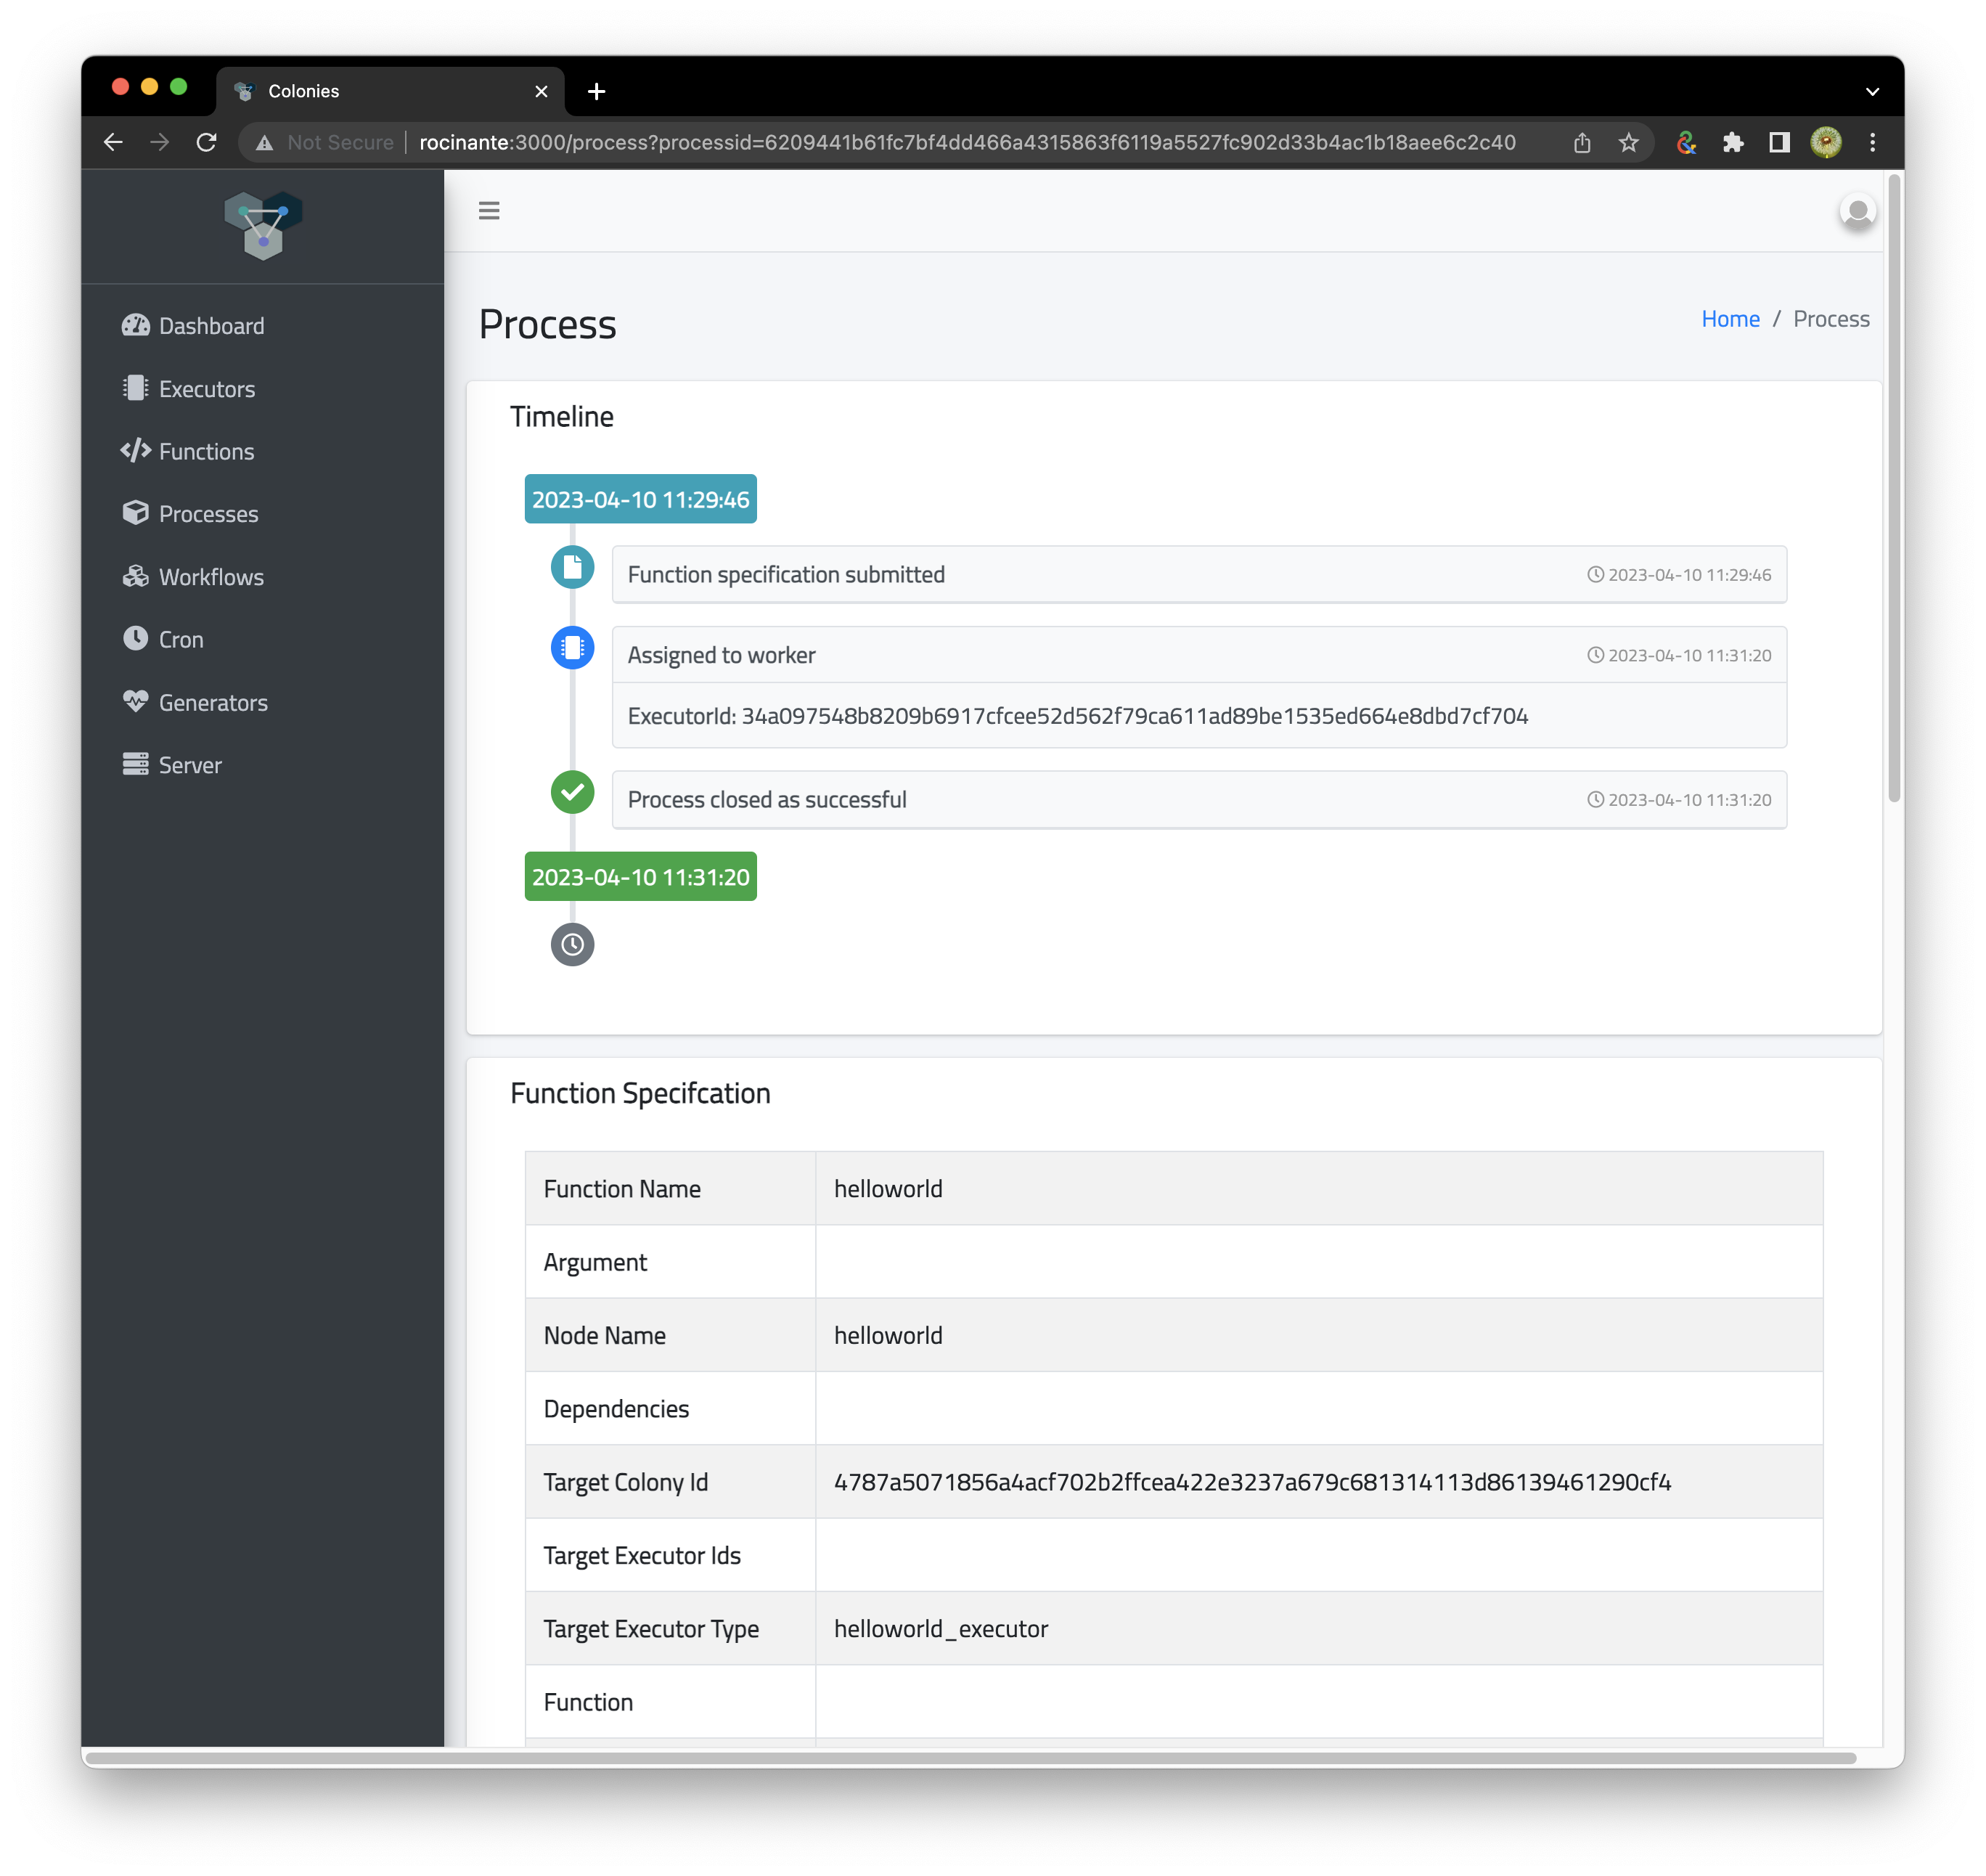
\includegraphics[scale=0.17]{dashboard1.png}
         \caption{Screenshot of process information.}
     	 \label{fig:dashboard1}
     \end{subfigure}
     \hfill
     \begin{subfigure}[b]{0.49\textwidth}
         \centering
         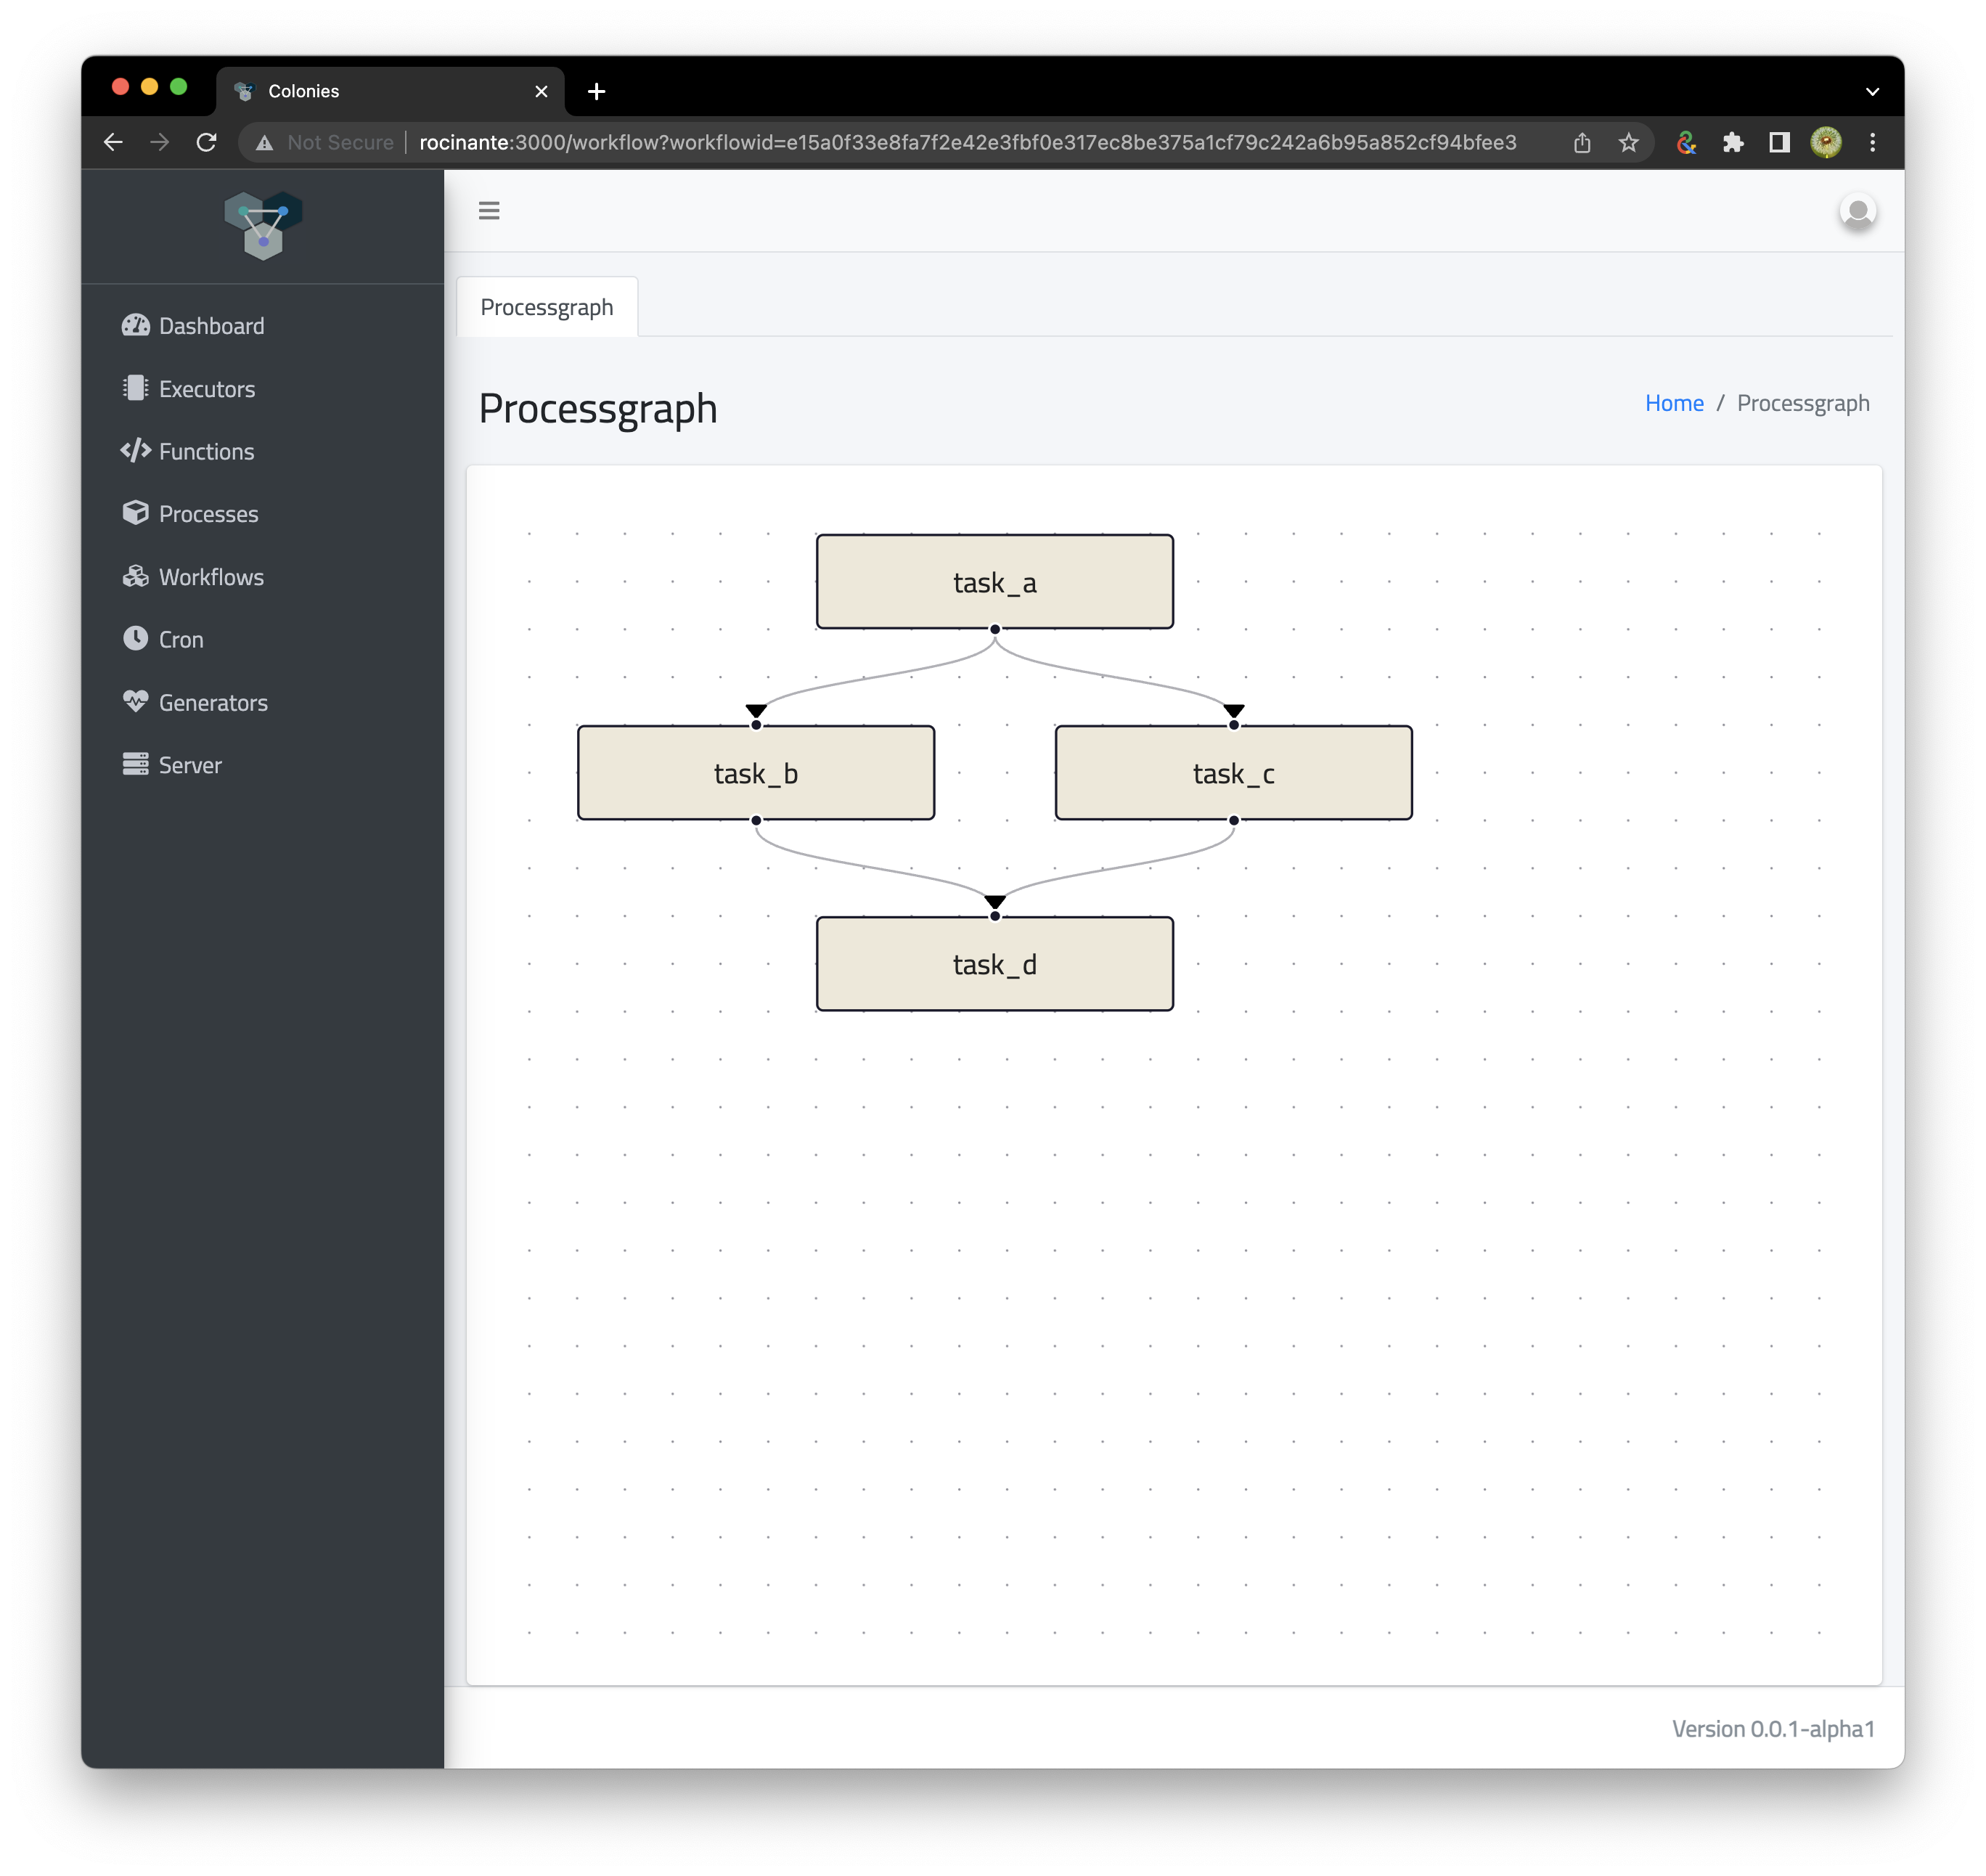
\includegraphics[scale=0.17]{dashboard2.png}
      	 \caption{Screenshot of a workflow.}
     	 \label{fig:dashboard2}
     \end{subfigure}
     \caption{Screenshot of the Colonies Dashboard tool.}
\end{figure}

% \begin{figure}[h]
% 	\centering
%     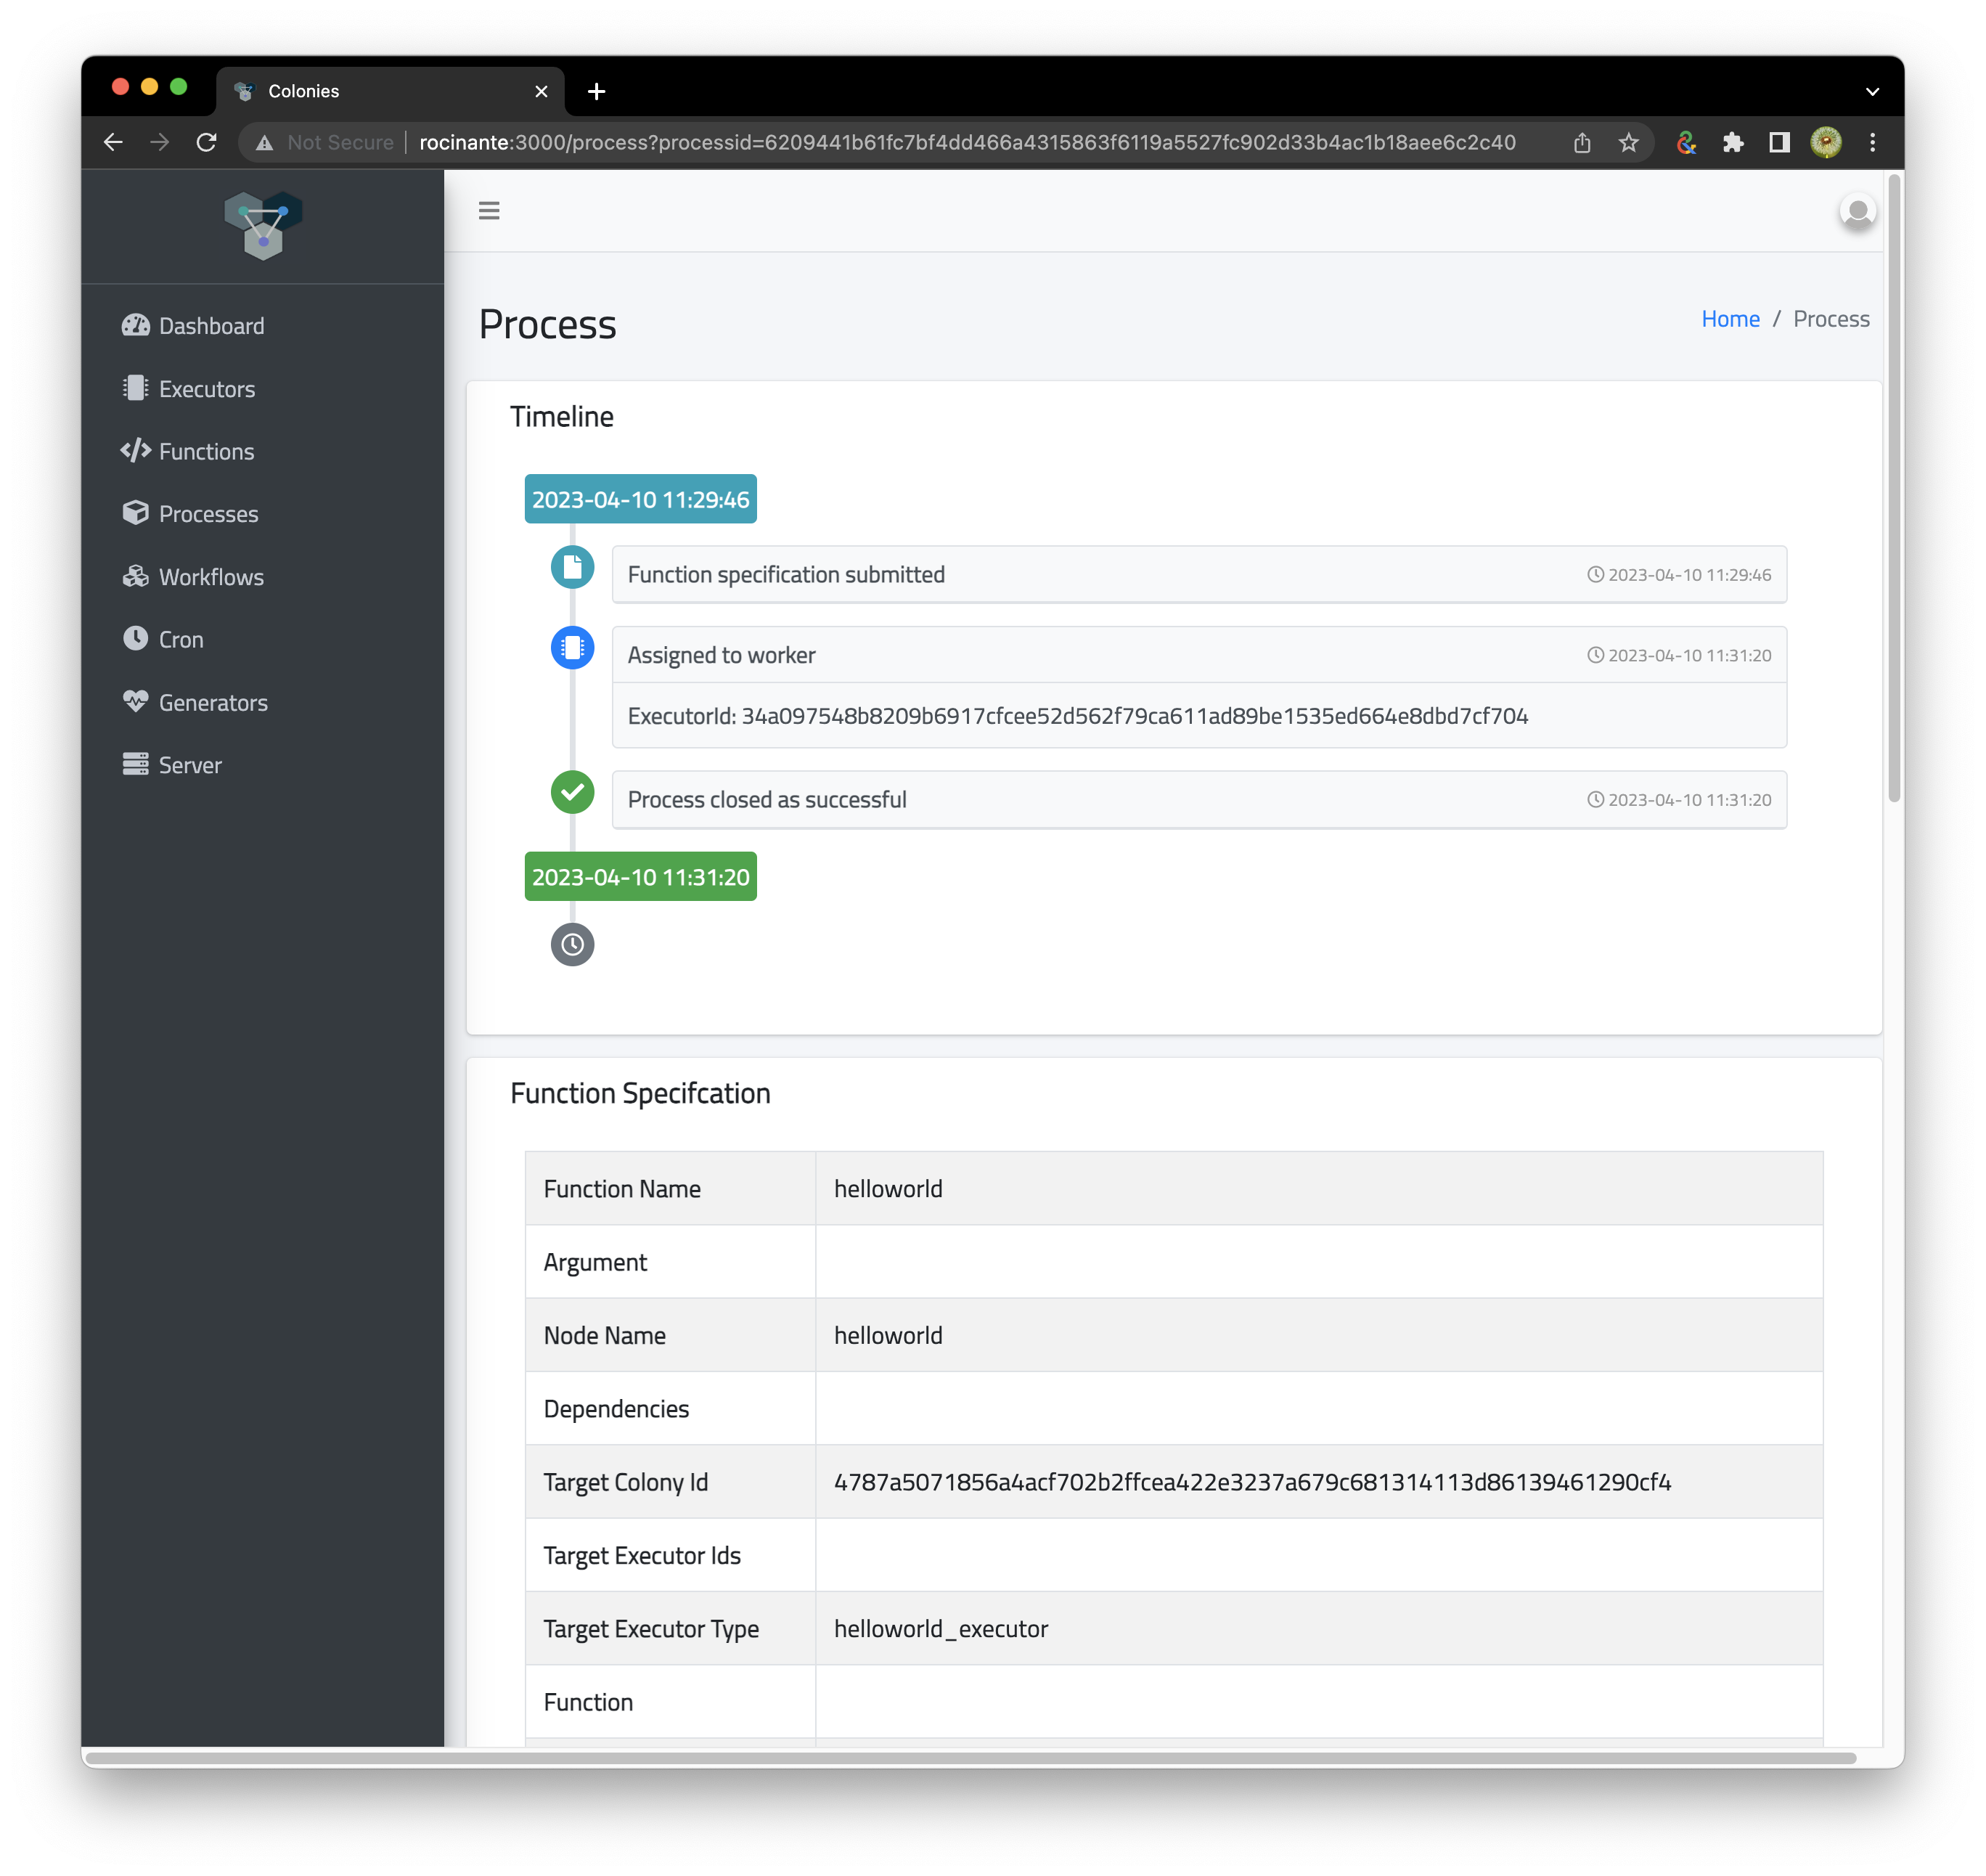
\includegraphics[scale=0.23]{dashboard1.png}
% 	\caption{Process information. The timeline makes it possible to follow the execution of process in realtime.}
% 	\label{fig:dashboard1}
% \end{figure}

Figure \ref{fig:dashboard1} shows a screenshot of the Colonies dashboard tool, which enables users to monitor the status of processes and executors. The timeline depicted in the figure allows for real-time monitoring of process execution, similar to tracking a physical package sent through a postal service. As previously discussed, it's also possible to subscribe to a process and receive information about its progress, which can be used as another point of integration. For example, sending a notification on Slack if a process fails.

\subsection{Workflows}
A workflow is just a set of processes with dependencies, which is represented as a DAG internally in Colonies. Workflows can either be submitted using SDKs or the Colonies CLI, which supports submission of JSON files. Listening \ref{code:workflow_spec} shows an example of a workflow consisting of four processes, each requiring different types of executors. The management of workflows is entirely handled by Colonies, and each executor executes only processes that are part of the graph for which it is responsible for. This approach significantly reduces the complexity of designing, implementing and operating large-scale AI applications and data pipelines. 

\begin{lstlisting}[basicstyle=\small, label=code:workflow_spec, language=json, basicstyle=\small, caption=Example of a workflow expressed in JSON.]
[ { "nodename": "task_a",
    "funcname": "echo",
    "conditions": { "executortype": "executor_type1", "dependencies": [] } },
  { "nodename": "task_b",
    "funcname": "echo",
    "conditions": { "executortype": "executor_type2", "dependencies": ["task_a"] } },
  { "nodename": "task_c",
    "funcname": "echo",
    "conditions": { "executortype": "executor_type3", "dependencies": ["task_a"] } },
  { "nodename": "task_d",
    "funcname": "echo",
    "conditions": { "executortype": "executor_type4", "dependencies": ["task_b", "task_c"] }
  } ]
\end{lstlisting}

% \begin{figure}[h]
% 	\centering
%     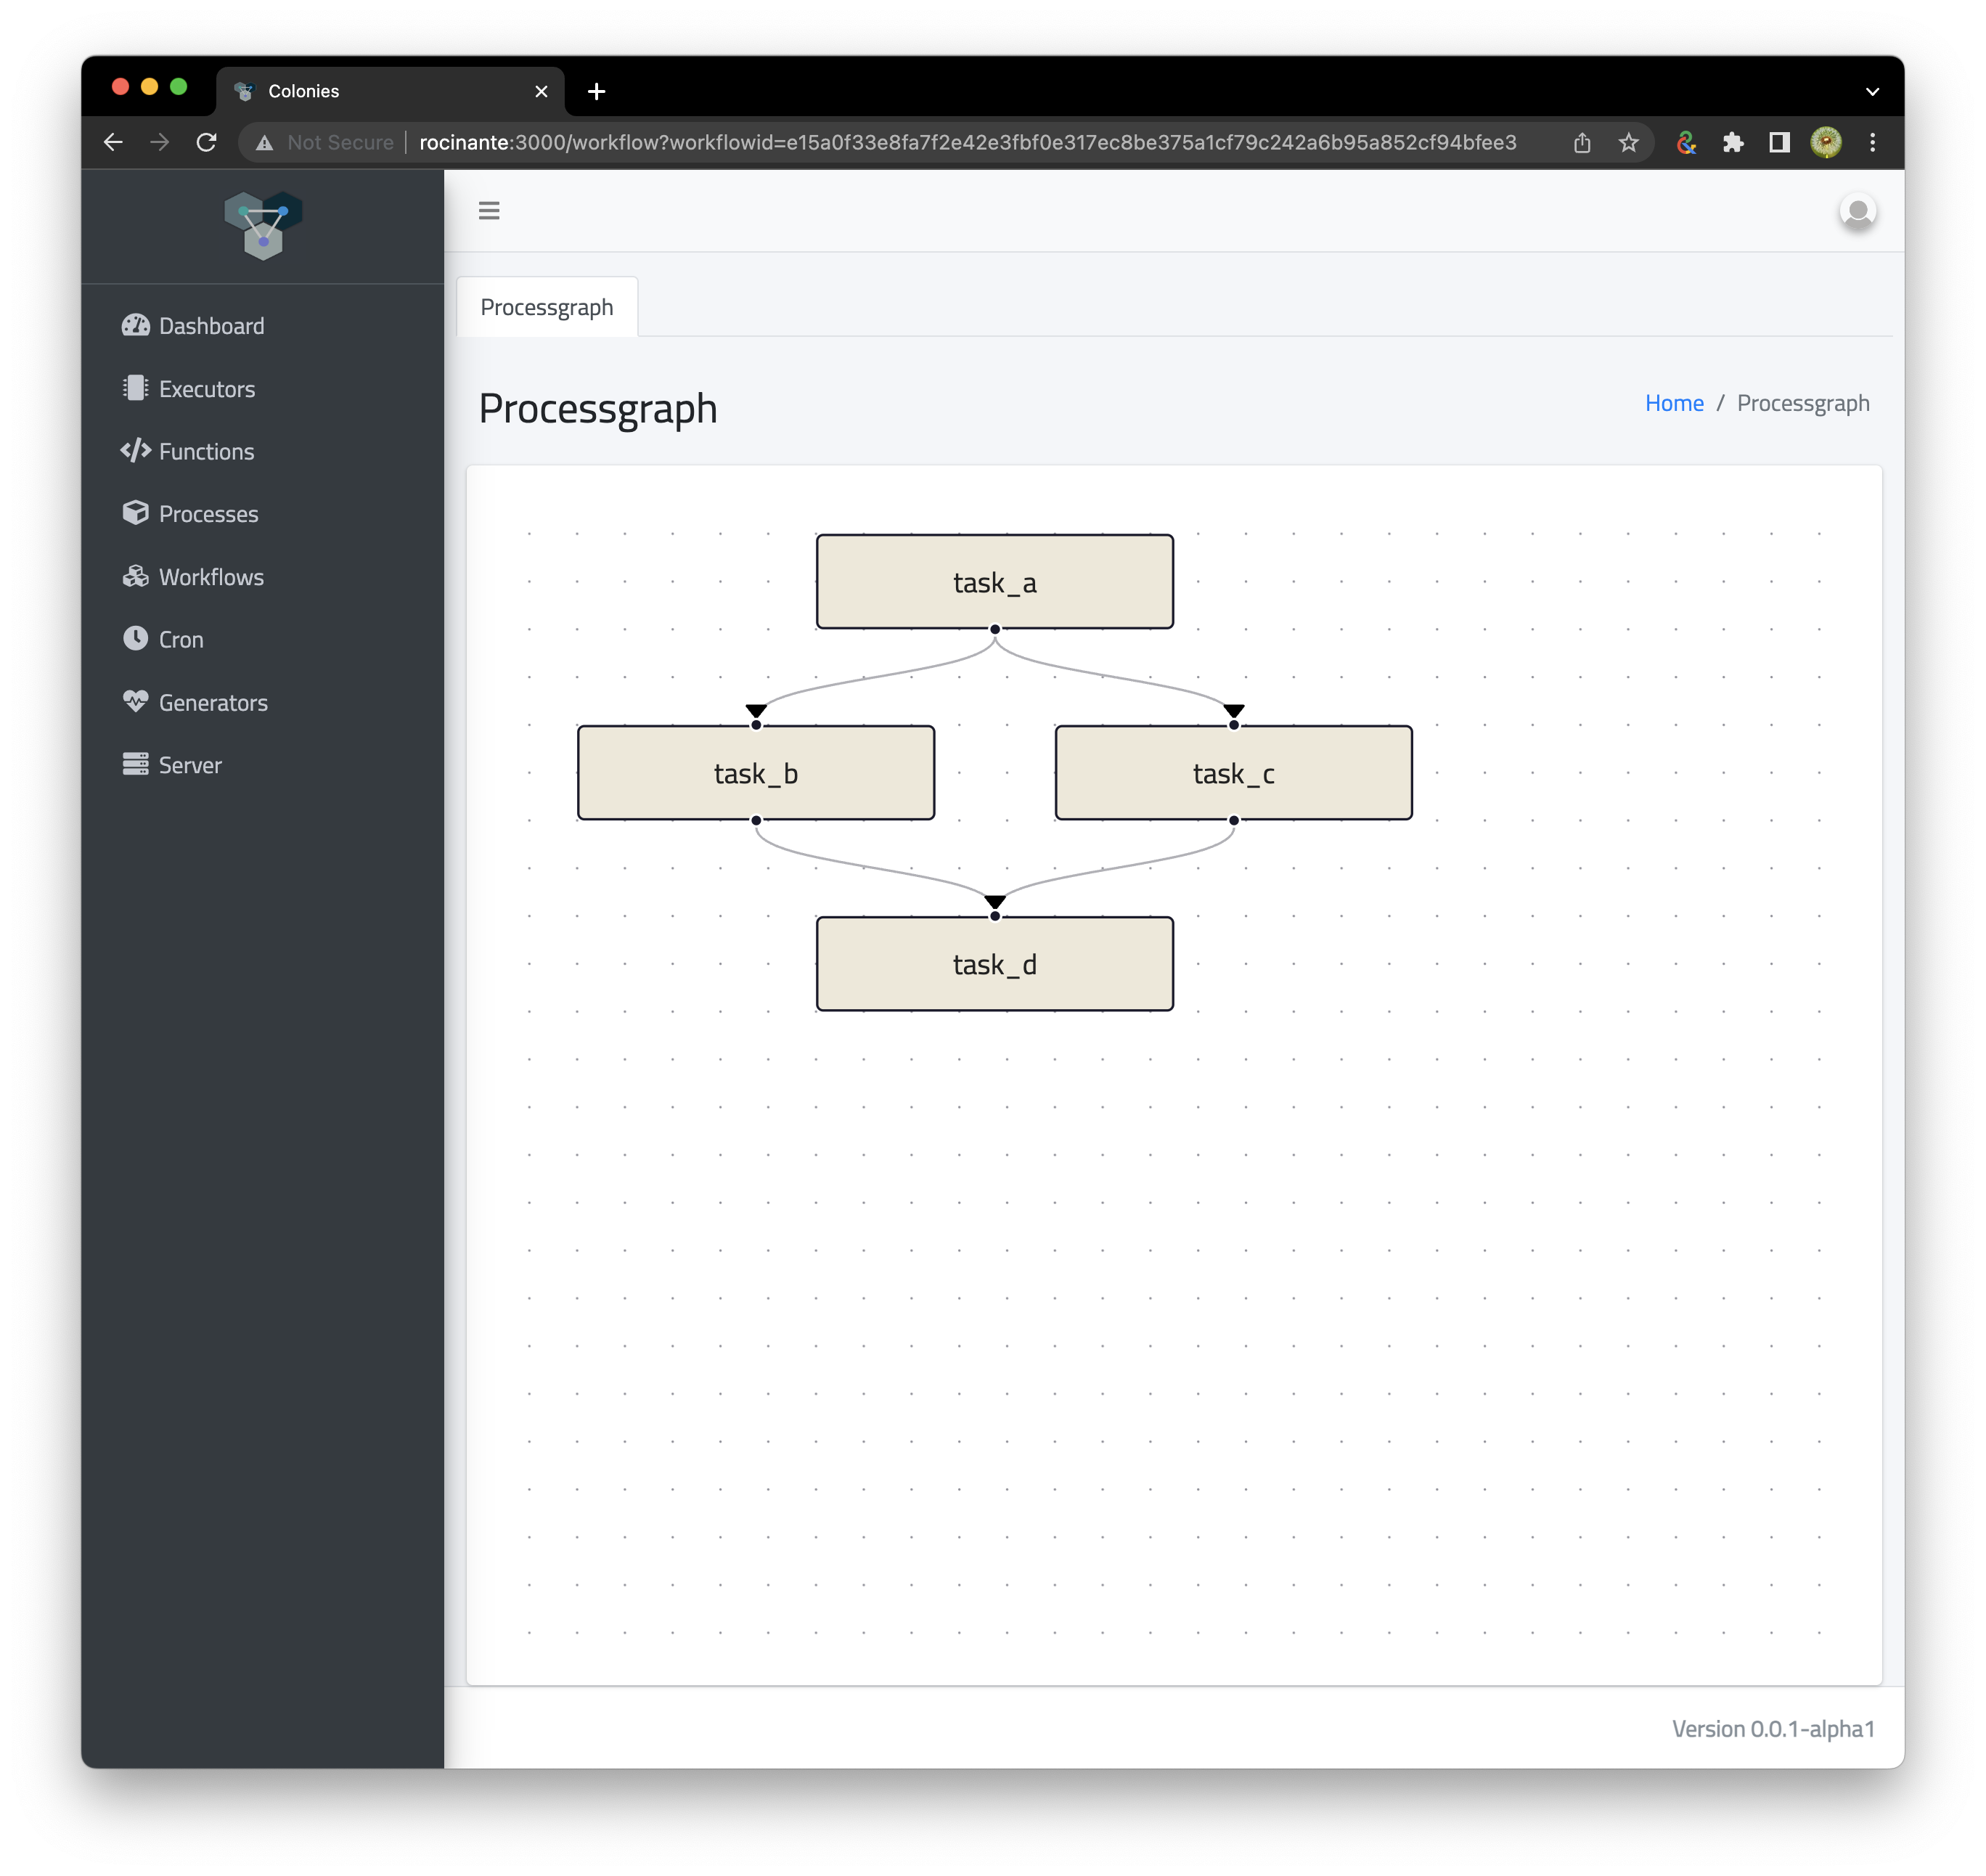
\includegraphics[scale=0.23]{dashboard2.png}
% 	\caption{Screenshot of a workflow in the Colonies dashboard.}
% 	\label{fig:dashboard2}
% \end{figure}

In addition to monitoring processes and executors, the Colonies dashboard can be used to visualize workflows. Figure \ref{fig:dashboard2} shows a DAG created when submitting the workflow code shown in Listing \ref{code:workflow_spec}. This functionality makes it possible to follow workflow execution progress.

\begin{figure}[h]
	\centering
    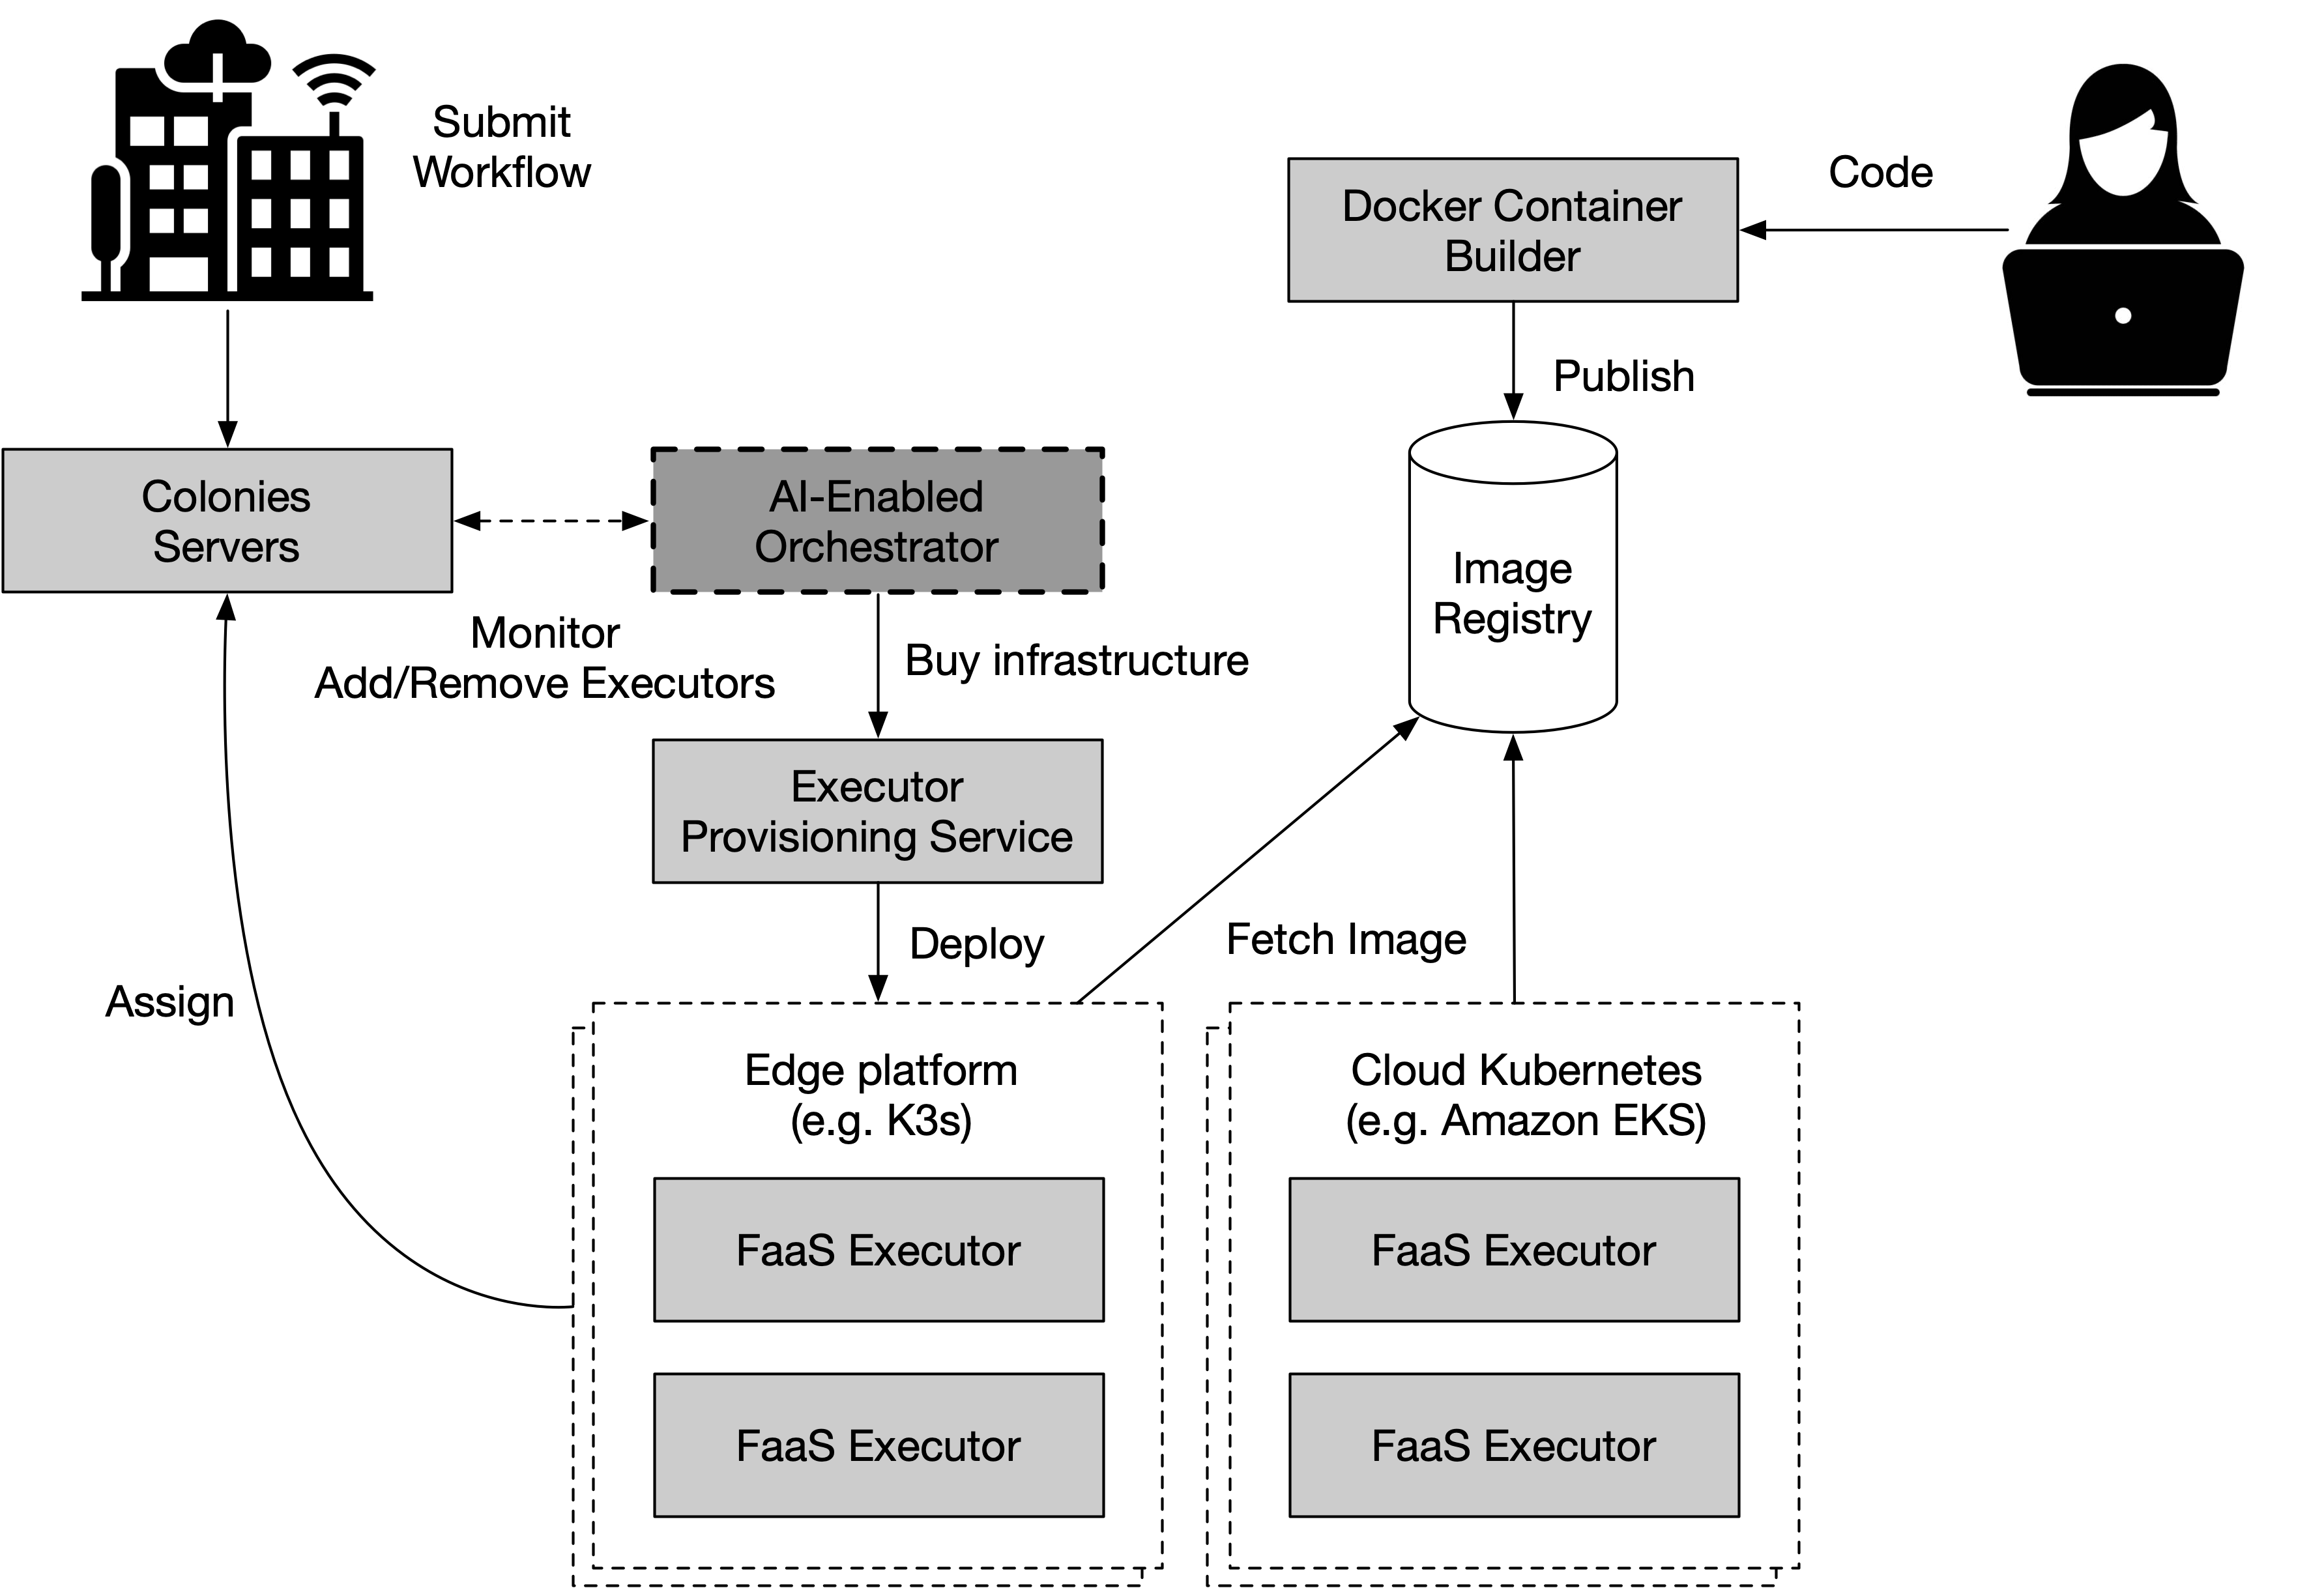
\includegraphics[scale=0.44]{cognite_faas.png}
	\caption{A Colonies-based FaaS serverless computing platform.}
	\label{fig:faas}
\end{figure}

\section{Use cases}
Colonies is currently used commerically by a startup company called RockSigma AB\footnote{https://www.rocksigma.com} to implement a compute engine for analysing seismic activities in underground mines. The paper will not explain the details of this specific implementation; instead it will outline other potential use cases where Colonies could make a considerable impact.

\subsection{Serverless computing}
\label{faas}
Serverless computing is a cloud-based architecture that allows developers to build and deploy applications without the need to manage the underlying infrastructure. In this model, the cloud service provider dynamically allocates and manages resources such as adding computing power or storage required by an application. Function-as-a-Service (FaaS) is a serverless computing model where developers provide code snippets that should be executed, and the cloud provider takes care of scaling, configuration and deployment of that code snippets. FaaS is often used in event-driven architectures where functions are triggered by specific events, thus eliminating the need to keep servers continuously running. The Cognit project \cite{cognit} aims to extend the FaaS concept by supporting geographically distributed edge servers in addition to cloud server resources. The project is also going to develop an AI-enabled orchestrator that can decide where to deploy FaaS code.

Colonies offer functionality to call functions in remote executors, a fundamental requirement to implement a FaaS platform. Colonies also provides mechanisms for service discovery and security isolation to prevent non-authorized function calls. In some cases, it could make sense to manually manage a colony by an administrator, and manually registering and deploying executors. Alternatively, a software solution could be developed to automatically deploy or undeploy executors. Such an approach would be very similar to a Function-as-a-Service (FaaS) platform.

Figure \ref{fig:faas} depicts a Colonies-based FaaS platform. Similar to AWS Lambda or Google Cloud Functions, developers would need to upload code snippets, which would then be packaged and published as Docker containers. To invoke a function, a function specification needs to be submitted to the Colonies server indicating which function to call. 

The advantage of using Colonies to implement a FaaS platform is that it introduces an extra level of separation and the possibility to develop a loosely coupled system. For example, if an executor is missing, the process is simply enqueued until a free executor becomes available. A software agent could then monitor pending processes on the Colonies server, predict the system load, and automatically deploy executors to meet the load, resulting in a highly efficient and scalable system. In the future, the AI orchestrator developed in the Cognit project could also be used together with Colonies to reduce energy consumption, or minimize network latency by utilizing edge servers.


\subsection{Edge computing}
Edge computing is a distributed computing model that brings computing resources closer to the source where data is generated to improve efficiency or reduce latency. In edge computing, computing and processing is usually done on the \emph{edge} of a network, such as at a server connected to a 5G base station. One could for example imagine a drone video surveillance use case where parts of a video processing pipeline run on an edge server. This approach would make it possible to execute complex AI models that would otherwise be difficult to run on a drone with limited computing capabilities.

Setting up a video pipeline is a complex problem. First, the drone must be able to discover nearby edge servers, make sure the edge server has sufficient resources, deploy some software components at the edge server, then start a video server and finally connect to the video server. Orchestrating such a workflow requires configuration and provisioning of computational resources across platforms. 

\begin{figure}[h]
	\centering
    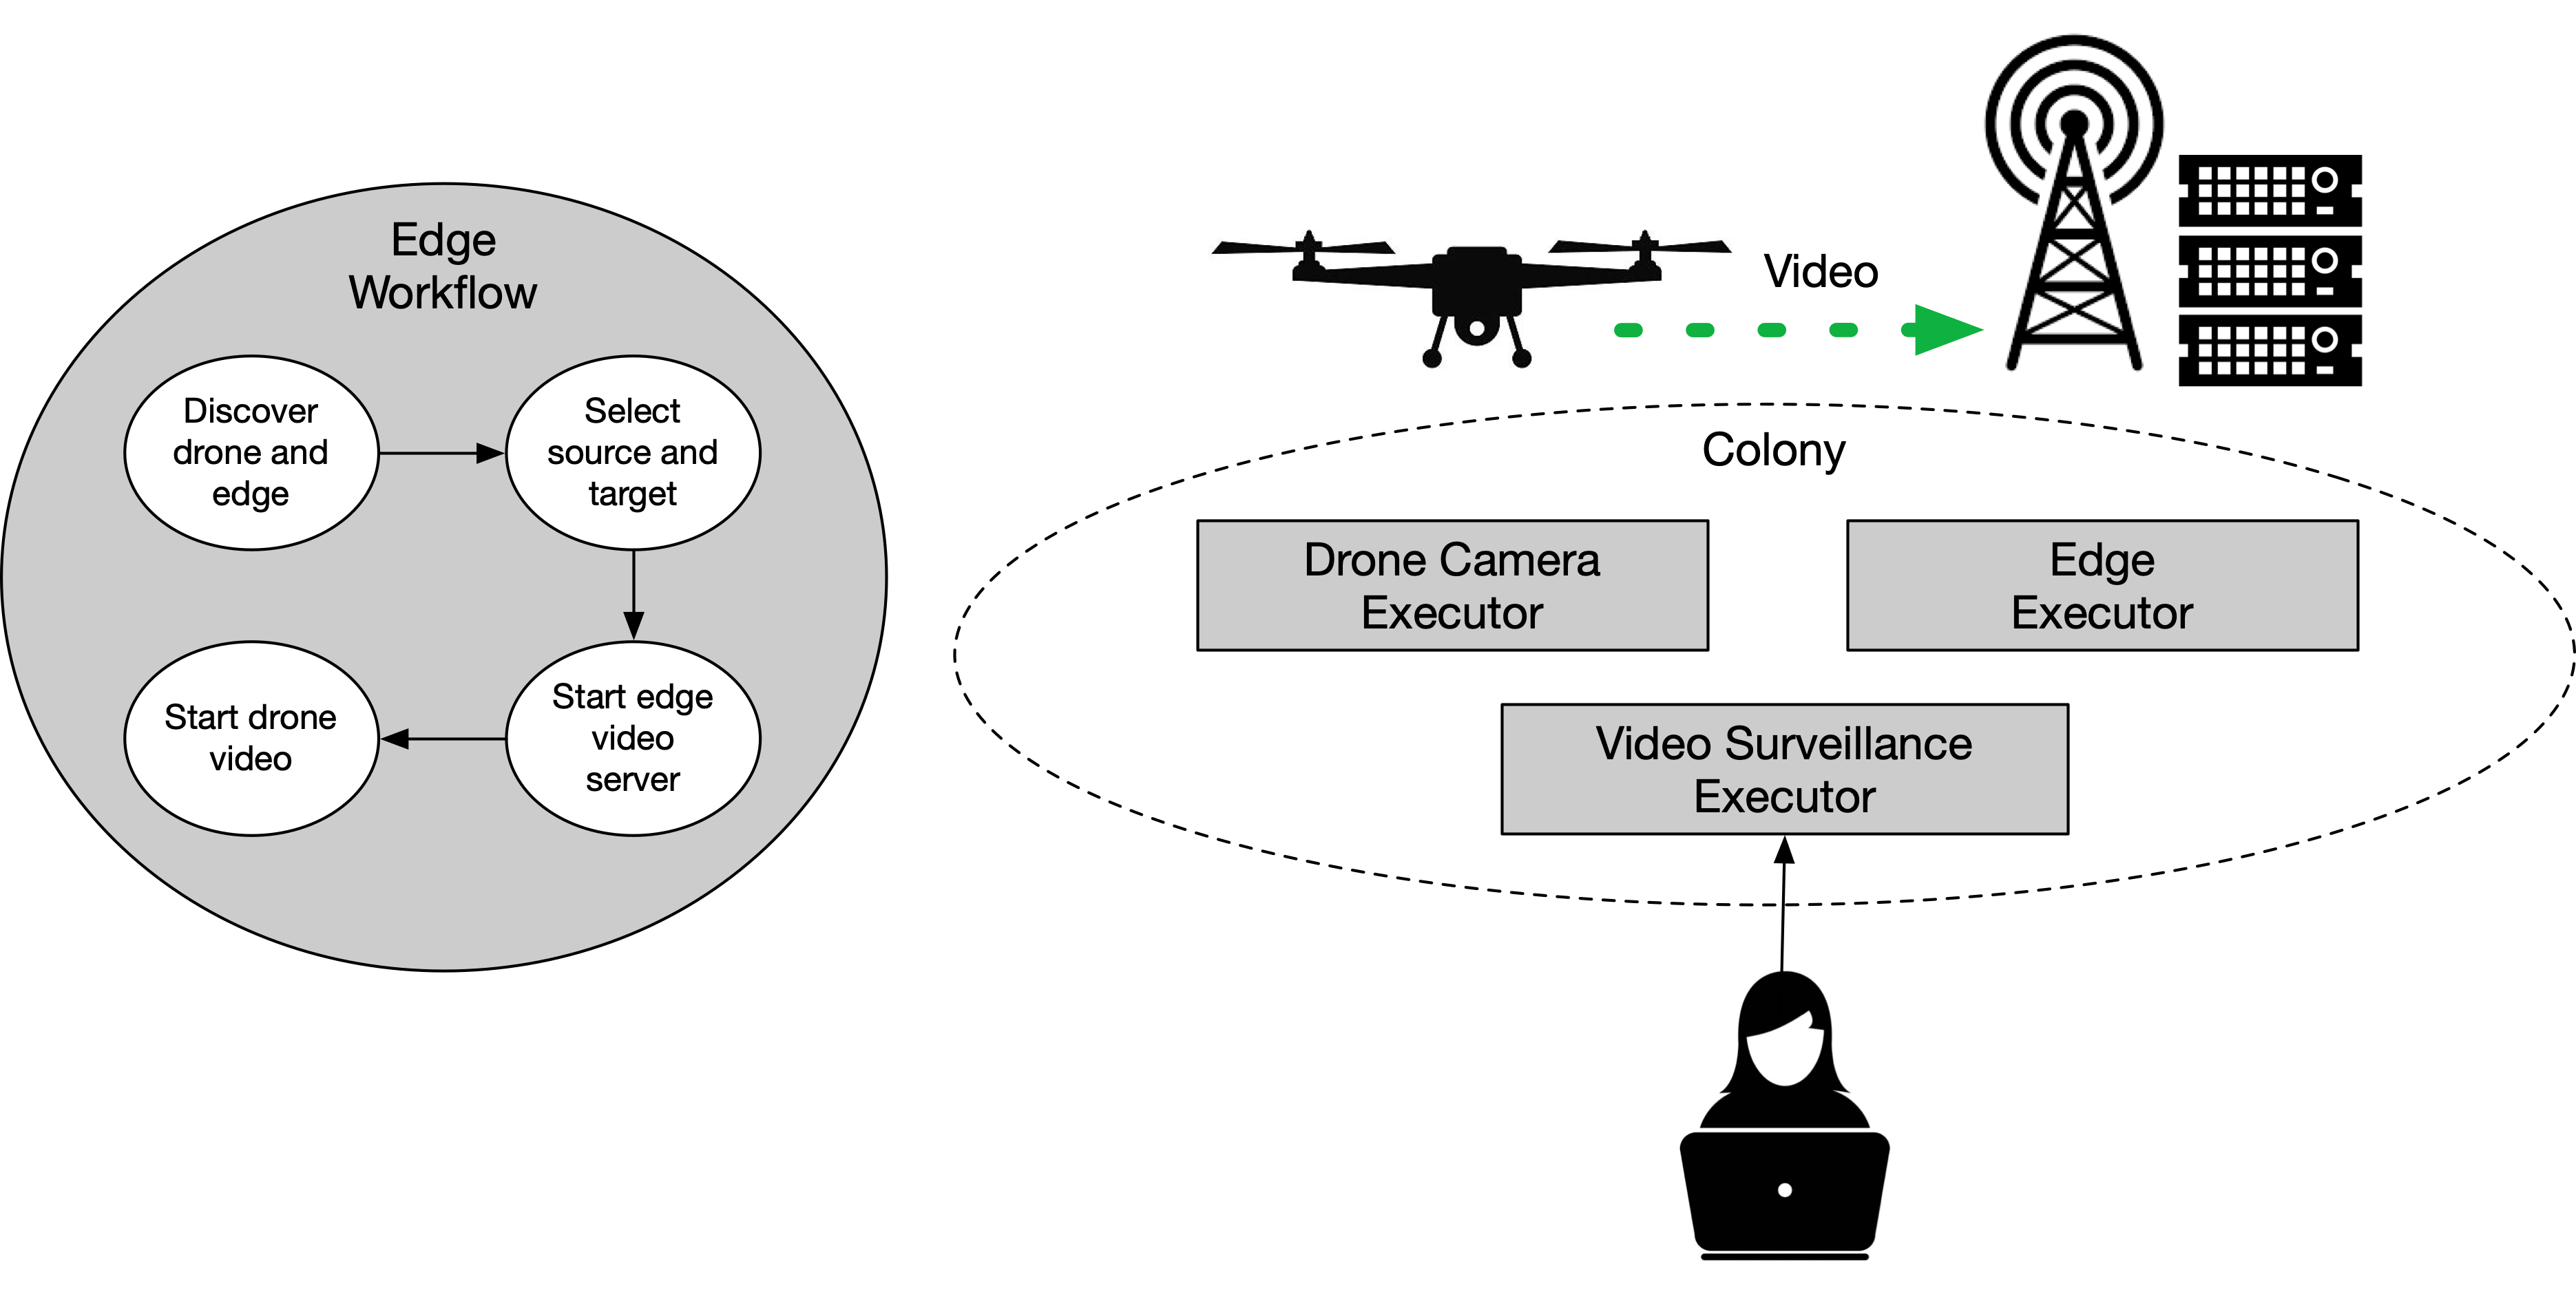
\includegraphics[scale=0.43]{edge.png}
	\caption{Edge workflows, using Colonies to control drones.}
	\label{fig:edge}
\end{figure}

The Colonies framework has the potential to streamline the setup of edge computing workflows by enabling devices and edge servers to be represented as distributed executors that can interact with other. Figure \ref{fig:edge} illustrates a setup of three executors. The \emph{Edge Executor} is responsible for deploying and setting up video processing software at an edge server, while the \emph{Drone Executor} is responsible for activating the video camera at the drone and establishing a connection to the video server hosted on the edge server. The \emph{Video Surveillance Executor} is responsible for identifying suitable edge servers and facilitating submission of workflows by users. Discovery of edge executors can be achieved by interacting with a Colonies server and searching the colony for available executors.

Figure \ref{fig:edge} also depicts a Colonies workflow. The workflow guarantees that the video pipeline is set up in the right order. For example, the drone executor should only connect to the edge server after the video server is running. The workflow can also be used to pass information between the executors. After the \emph{Edge Executor} has set up a video server, it sends a \emph{close} request containing the IP address to the video server. The IP address will then be passed as input to the next process in the workflow, allowing the \emph{Drone Executor} to establish a connection to the edge server.

\subsection{High-performance computing}
\label{hpc_use_case}
Slurm \cite{slurm} is a workload manager and job scheduler commonly used in HPC environments. In contrast to Colonies, it provides functionality to reserve resources. This is particularly useful when running complex simulations that require a large number of CPUs or a large amount of memory. 

A challenge associated with Slurm and HPC environments in general is that they can be difficult to set up and use. Submitting a job typically requires users to develop job scripts and manually transfer data to the HPC environment before a job can be executed. Compared to cloud platforms, Slurm is less mature when it comes to API and automation support, which can make the usage more time-consuming and manual.

\begin{figure}[h]
	\centering
    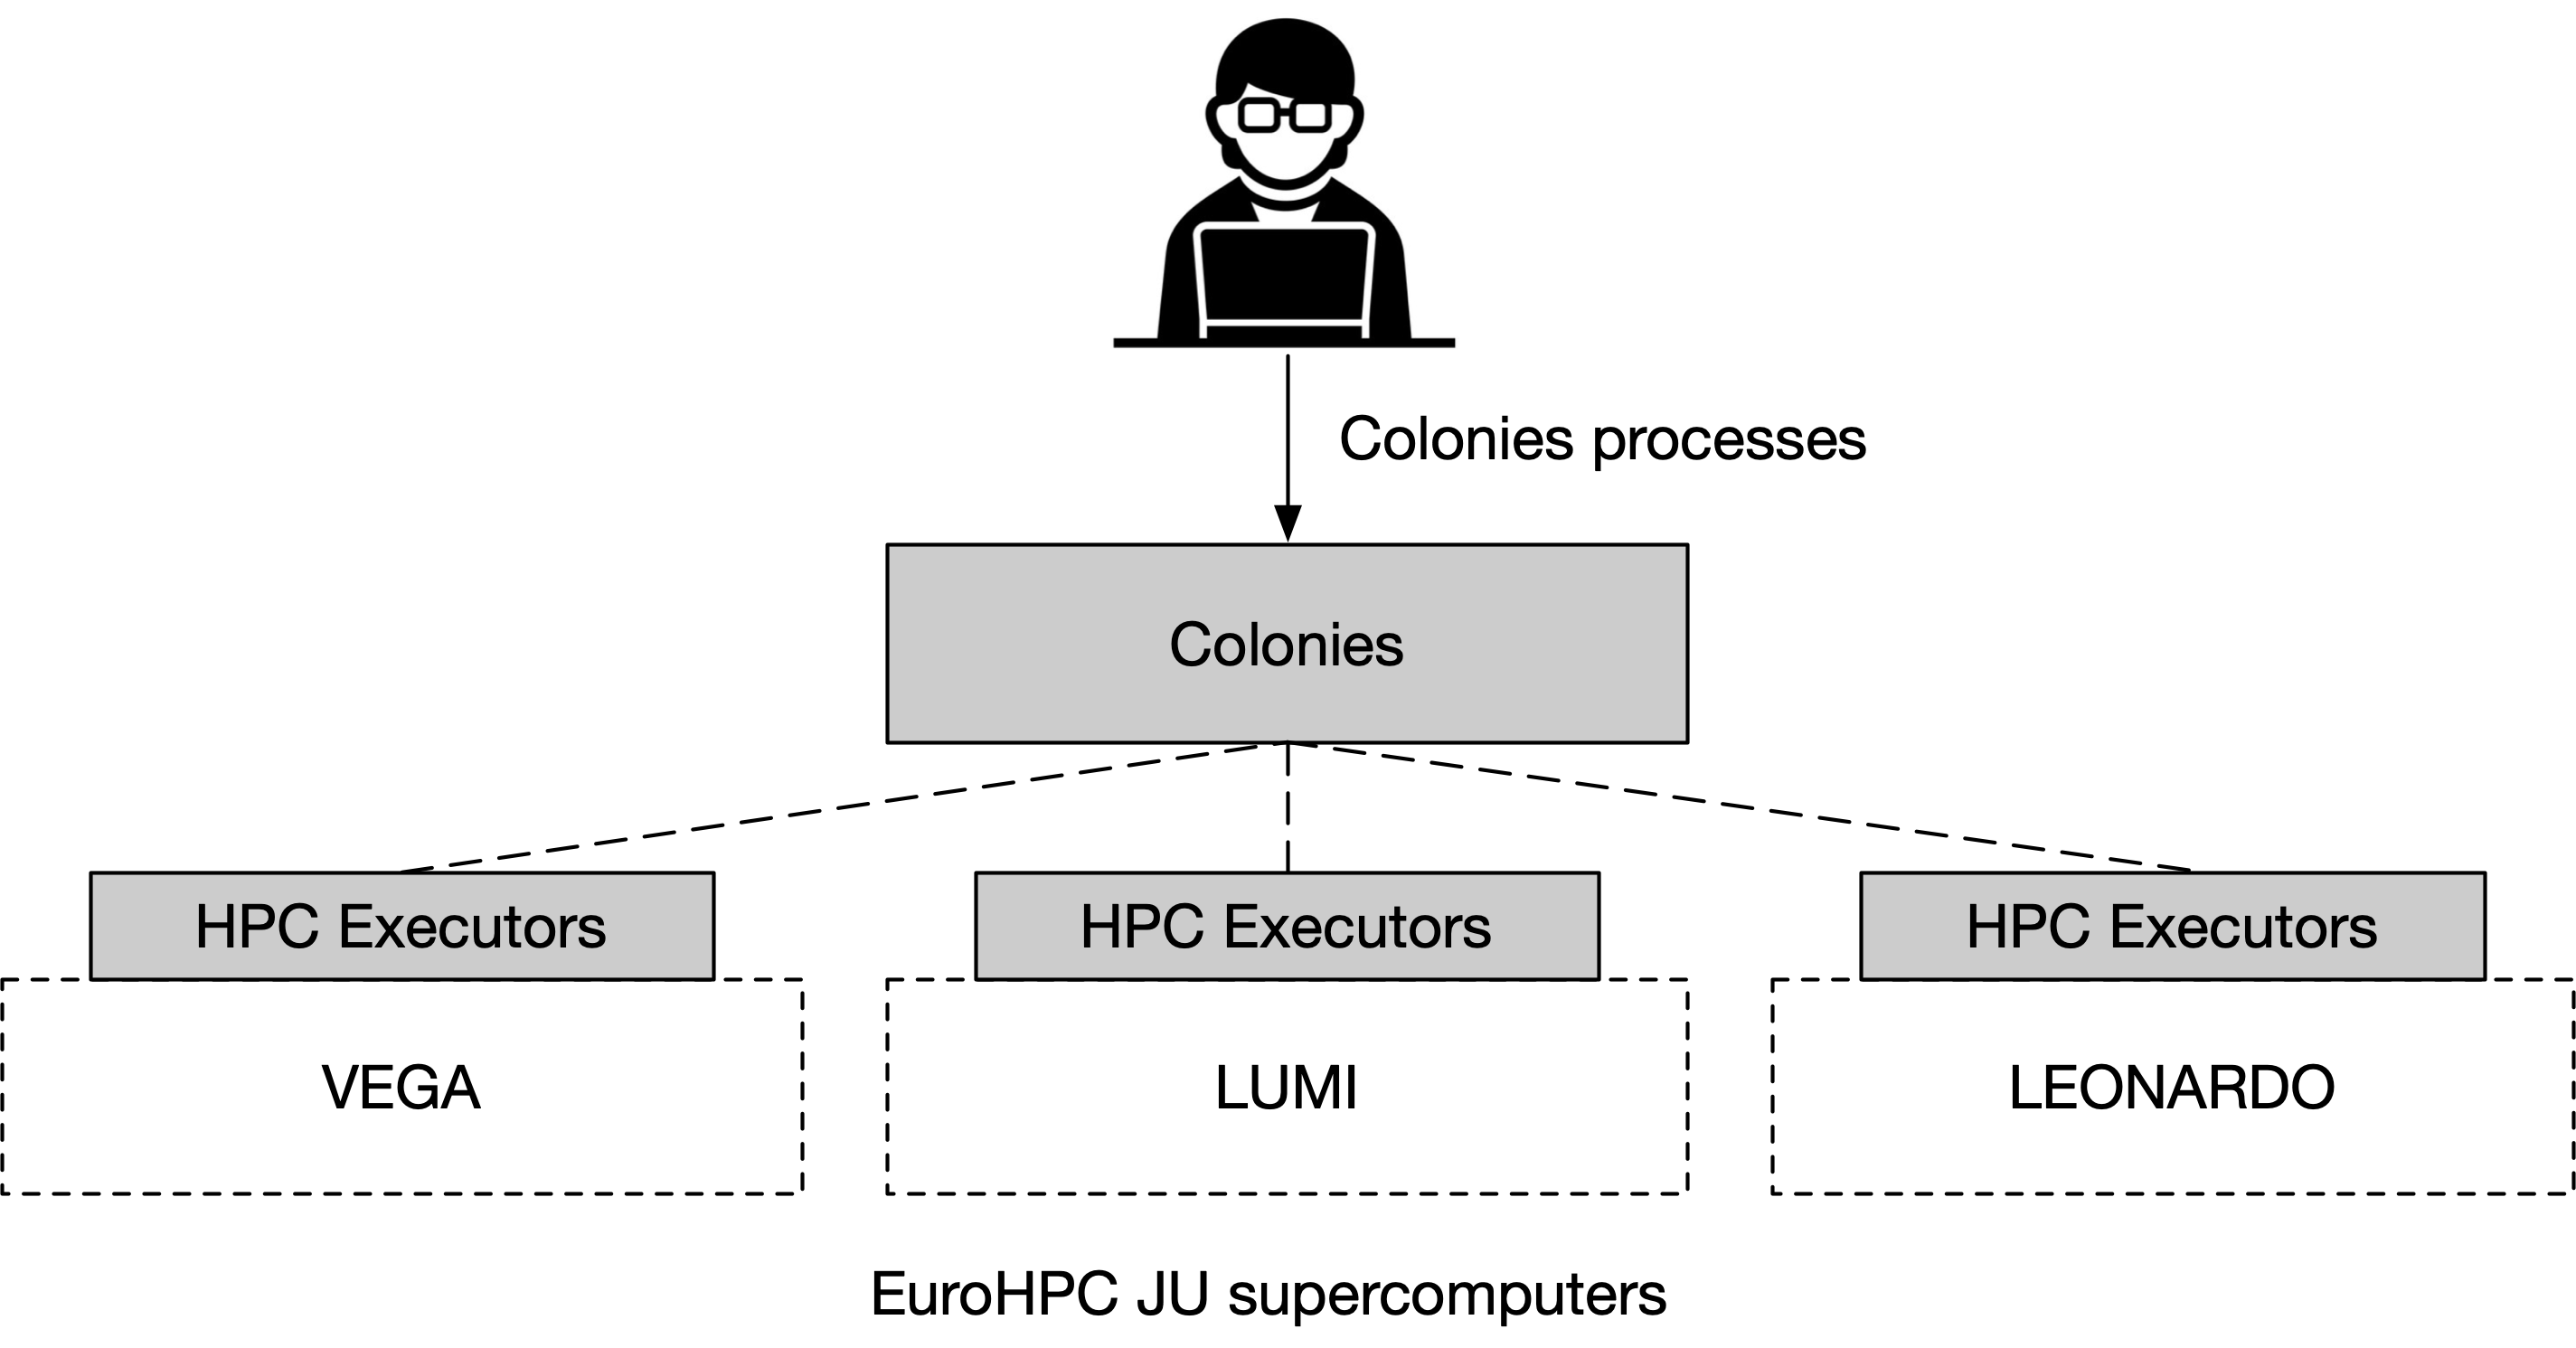
\includegraphics[scale=0.43]{hpc_overlay.png}
	\caption{A Colonies-based submission system for HPC.}
	\label{fig:hpc_overlay}
\end{figure}

Colonies could be used to fill the gap between cloud and HPC and create workflows that can partly run in cloud while also taking advantage of the vaste computational capacity offered by HPC. For example, a company could develop a workflow that automatically copy training data to a HPC center, train a neural network, move the result back to the cloud, and finally re-deploy a Kubernetes service to use the new model. With Colonies, users can indirectly control HPC systems by submitting Colonies processes that are subsequently picked up by HPC executors, without requiring direct connection to the HPC system. Essentially, using Colonies as a cloud-based submission system for HPC connecting different HPC centers together. Figure \ref{fig:hpc_overlay} depicts such a submission system.

Figure \ref{fig:hpc_workflow} shows an example how Colonies could be used in a HPC environment. Several executors run at the HPC system, each with their own responsibilities. The \emph{Container Importer Executor} is responsible for converting container images to a format that is supported by Slurm, e.g. Singularity containers\footnote{https://docs.sylabs.io}. The \emph{Data Importer Executor} downloads data to the HPC file system. The \emph{Slurm Executor} is responsible for submitting and overseeing Slurm jobs, while the \emph{Data Exporter} executor is responsible for uploading result data to the cloud.

\begin{figure}[h]
	\centering
    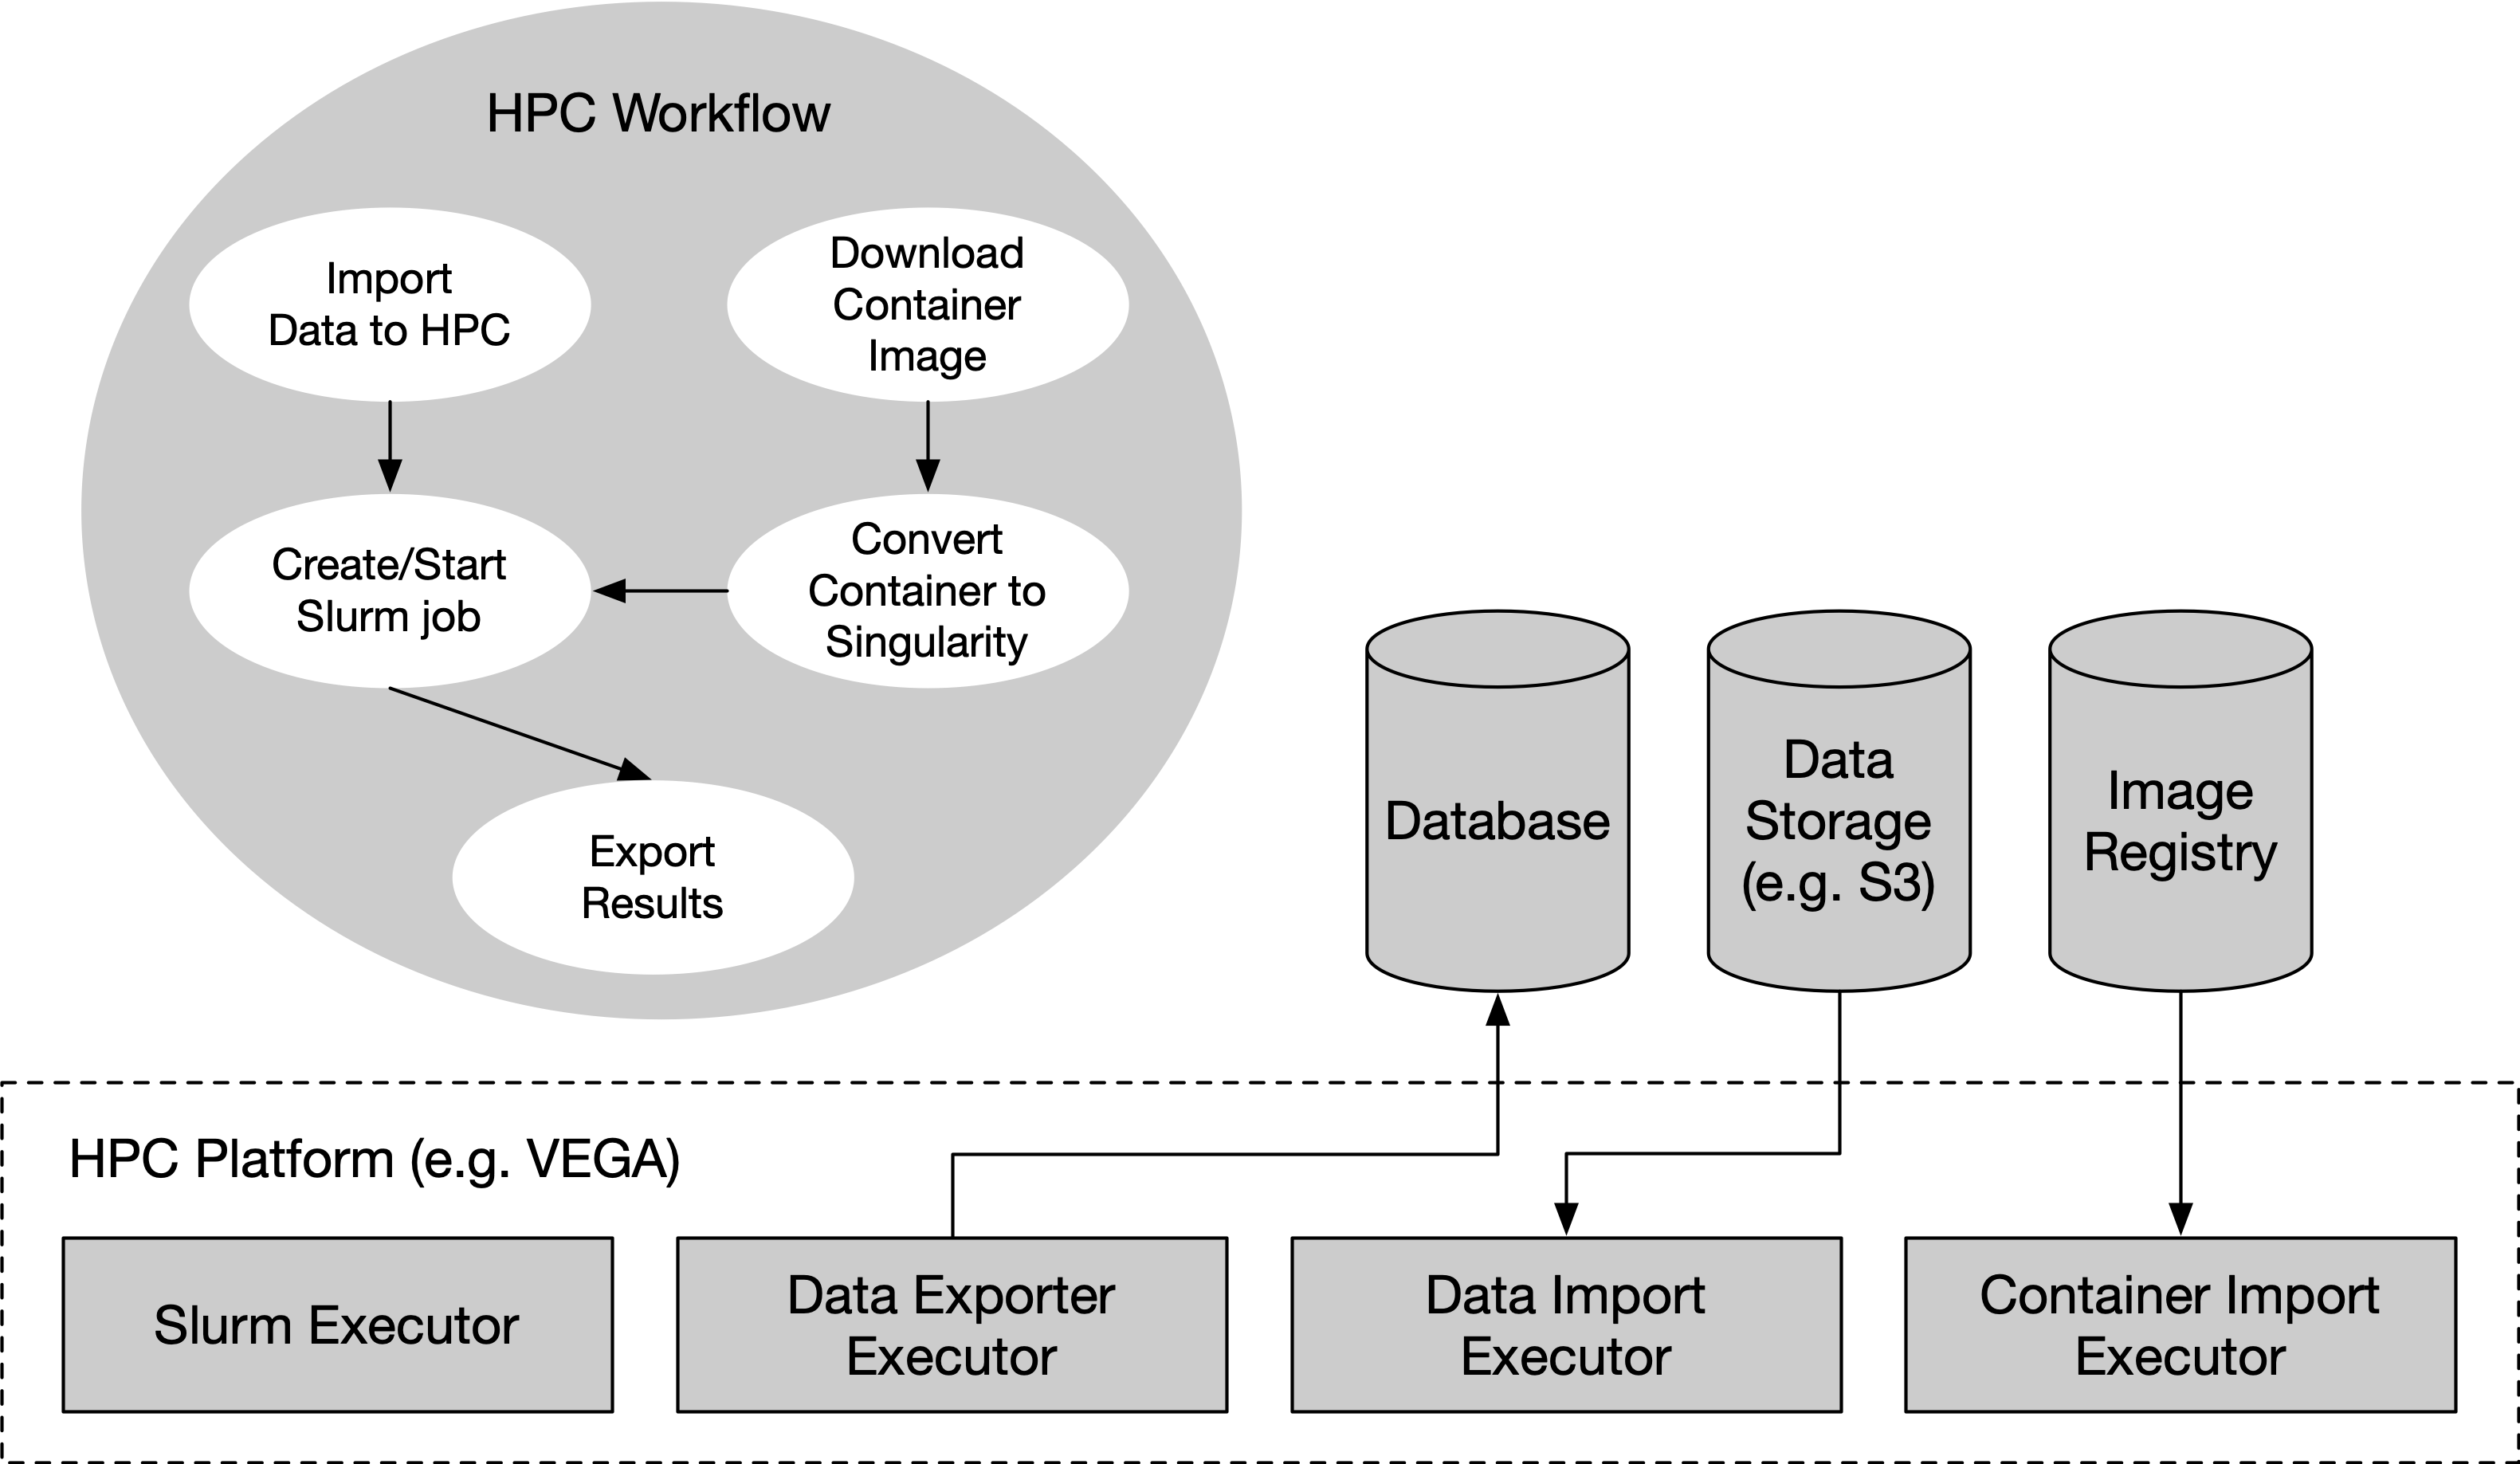
\includegraphics[scale=0.43]{hpc_workflow.png}
	\caption{HPC workflow.}
	\label{fig:hpc_workflow}
\end{figure}

% \subsection{Earth Observation}
% OpenEO \cite{openeo} is an open-source project that aims at providing a standardized and interoperable solution for accessing, processing, and analyzing Earth observation (EO) data. Its primary objective is to facilitate seamless user interaction with diverse data sources and processing backends through a unified API. An overview of various OpenEO backends is presented in \cite{openeo_backends}. The paper concludes that there is a need for a more decentralized and federated EO data processing platform, and OpenEO represents a significant step in this direction. Nevertheless, the paper also acknowledges that the implementation of underlying datacubes, storage solutions, and service plans cannot be entirely abstract away by the OpenEO API.

% \begin{figure}[h]
% 	\centering
%     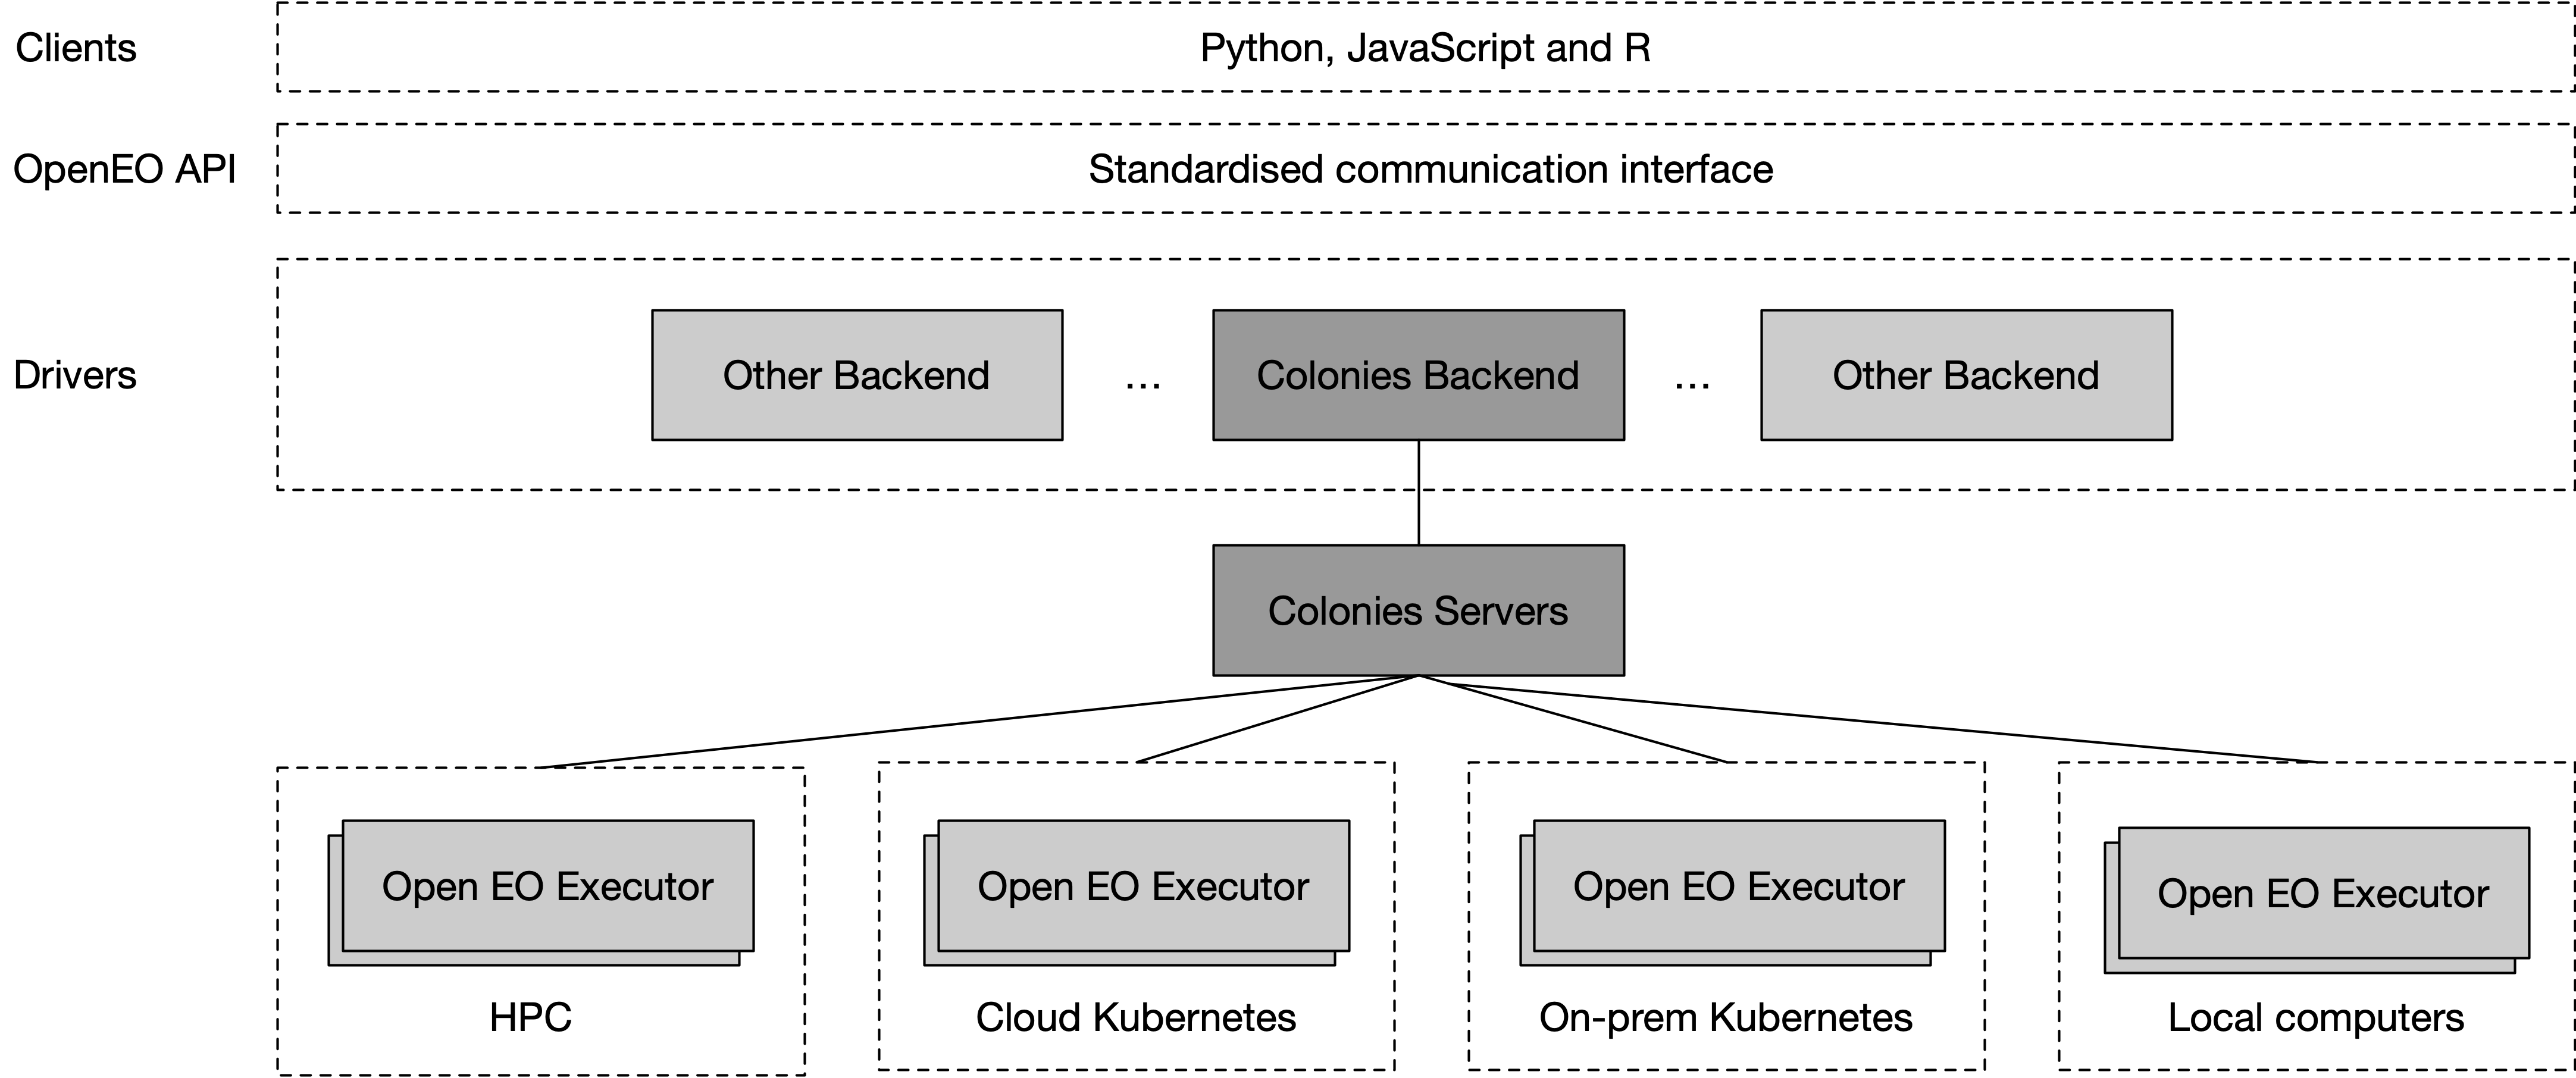
\includegraphics[scale=0.43]{openeo.png}
% 	\caption{OpenEO integration}
% 	\label{fig:dashboard2}
% \end{figure}

% Colonies can be used to implement a decentralized grid-based compute infrastructure for Earth Observation (EO) workloads across diverse platforms. By wrapping computational EO tasks into Colonies processes, interoperability among platforms can be further enhanced. For instance, it becomes possible to create a broker-based architecture that enables OpenEO applications to submit job specifications indirectly to a Colonies server. These specifications could then be picked up by executors connected to different backend providers. Executors could also be used to automatically provision compute resources. For example, automatically setting up Dask\footnote{https://www.dask.org} clusters, or deploy workflows at HPC systems to handle high-demand EO workloads. 

\section{Discussion}
This paper has presented an open-source framework called Colonies designed to streamline execution of computational workloads across platforms. Colonies provides a \emph{distributed runtime environment}, called a \emph{Colony}, which serves as an intermediary layer to indirectly control other computer systems. Instead of directly connecting different systems together, Colonies allows services or users to publish instructions and then assign these instructions to other services. By chaining instructions together, it becomes possible to execute workloads that can operate seamlessly across different platforms. 

Colonies builds on the principle: \emph{security first}. Public key encryption allows administrators and users to maintain strict control over a colony, even when executors are dispersed throughout the Internet. Each colony is governed by a private key that serves as a central authority, analogous to \emph{one ring to rule them all}, making it possible to control a colony as if it was a single machine. The zero-trust principle, \emph{trust, but verify} also enables development of immune system-like functionality where malfunctional executors can be excluded and replaced with fresh new ones, ensuring that the overall performance and reliability of the system is not compromised. 

A significant portion of the paper has focused on describing how to handle robustness to allow software components to fail without compromising the entire system. A critical design decision that makes Colonies robust and scalable is its stateless architecture. Colonies also make sure that workflow execution runs to completion, even if some executors fail. This makes it possible to implement robust data pipelines, but also efficiently handle IT operations such as continuous deployments and software updates. Both security and robustness are crucial factors to consider when developing a workflow management system that is capable of functioning across platforms and handling constantly changing infrastructures. 

It has been mentioned in the paper several times that Colonies is designed to simplify integration with other systems. Microservices is a design principle used by Colonies to simplify integration. As executors are designed to be loosely-coupled microservices, the entire system becomes easier to develop, test, and maintain. For example, different teams can take on responsibility to develop a certain executor, which can then be used as a part of complex workflows running across platforms. By designing each executor as a standalone microservice, it also becomes easy to scale the system by simply deploying more executors. This also opens up for an intriguing possibility to delegate colony management responsibility to a software agent that can automatically provision and deploy executors on demand.

While microservices is a powerful design pattern, Colonies goes beyond the conventional microservice model and offers a distributed microservice architecture allowing microservices to reside anywhere on the Internet. Also, by acting as an intermediary layer, Colonies provides a unified interface to facilitate interaction between these microservices, ultimately making it possible to create workflows that span multiple platforms. The paper has also presented into several use cases related to edge computing, cloud computing and high-performance computing, highlighting the benefits that such a framework could provide, in particular how to create loosely-coupled systems that offers both flexibility, robustness, and scalability.

To sum up, the long-term vision of the Colonies framework is to offer uninterrupted access to computing resources, allowing data to flow from one service to another. Achieving seamless compute continuum requires development of simple, secure, scalable, and robust solutions. Colonies serves as an initial step towards realizing this vision of a seamlessly integrated computing ecosystem.

\bibliographystyle{unsrt}
\bibliography{references} 

\newpage
\appendix
\section{Appendix - Colonies Operations}
\begin{table}[h]
	\centering
	\begin{tabular}{llcl}
		\toprule
		\cmidrule(r){1-4}
        Operation                  & Role         & Assign required & Note \\
		\midrule
        \(add\_colony\)            & Server owner &            & Registers a new colony. \\
        \(delete\_colony\)         & Server owner &            & Unregisters a colony. \\
        \(add\_executor\)          & Colony owner &            & Register a new executor to a colony. \\
        \(delete\_executor\)       & Colony owner &            & Unregister a executor from a colony. \\
        \(approve\_executor\)      & Colony owner &            & Approve an executor. \\
        \(reject\_executor\)       & Colony owner &            & Disaprove an executor. \\
        \(get\_executors\)         & Executor     &            & List all executors member of a colony. \\
        \(get\_executor\)          & Executor     &            & Get info about an executor. \\
        \(get\_colonies\)          & Executor     &            & List all colonies on the Colonies server. \\
        \(get\_colony\)            & Executor     &            & Get info about a colony. \\
        \(subscribe\_process\)     & Executor     &            & Subscribe to a particular process. \\
        \(subscribe\_processes\)   & Executor     &            & Subscribe to processes status changes. \\
        \(submit\)                 & Executor     &            & Submit a function specification. \\
        \(assign\)                 & Executor     &            & Assign a waiting process to an executor. \\
        \(unassign\)               & Executor     & x          & Unassign a process from a executor. \\
        \(close\)                  & Executor     & x          & Close a process as successful. \\
        \(fail\)                   & Executor     & x          & Close a process as failed. \\
        \(get\_processes\)         & Executor     &            & List waiting, successful or failed processes. \\
        \(get\_process\)           & Executor     &            & Get info about a process. \\
        \(delete\_all\_processes\) & Colony owner &            & Delete all processes. \\
        \(delete\_process\)        & Colony owner &            & Delete a process. \\
        \(add\_attribute\)         & Executor     & x          & Add attribuite to a process. \\
        \(remove\_attribute\)      & Executor     & x          & Remove attribute from a process. \\
        \(subscribe\_attribute\)   & Executor     &            & Subscribe to a attribute. \\
        \(submit\_workflow\)       & Executor     &            & Submit a workflow. \\
        \(get\_workflow\)          & Executor     &            & Get info about a workflow. \\
        \(get\_dag\)               & Executor     &            & Get info about a DAG. \\
        \(add\_child\)             & Executor     & x          & Add a child to a process part of a DAG. \\
        \(add\_generator\)         & Colony owner &            & Add a generator. \\
        \(get\_generators\)        & Executor     &            & Get info about a generator. \\
        \(pack\)                   & Executor     &            & Add input to an a generator. \\
        \(remove\_generator\)      & Colony owner &            & Remove a generator. \\
        \(add\_cron\)              & Colony owner &            & Add a cron to a colony.\\
        \(remove\_cron\)           & Colony owner &            & Remove a cron from a colony.\\
        \(get\_cron\)              & Executor     &            & Get info about a cron. \\
        \(delete\_cron\)           & Colony owner &            & Delete a cron from a colony.\\
        \(get\_crons\)             & Executor     &            & List all crons part of a colony.\\
        \(add\_function\)          & Executor     &            & Register a function to an executor. \\
        \(remove\_function\)       & Executor     &            & Unregister a function from an executor. \\
        \(get\_functions\)         & Executor     &            & List all functions supported by the colony. \\
		\bottomrule
	\end{tabular}
	\label{optable}
\end{table}

\end{document}
